% This document provides the style to be used for a MSc Thesis at the
% Parallel and Distributed Systems group
\documentclass[11pt,twoside,a4paper,openright]{report}

% use babel for proper hyphenation
%removed ducth babel language, I won't be using dutch anyway
\usepackage[english]{babel}
% Graphics: like the DUT logo on the front cover
\usepackage{graphicx}
% FONT: times
\usepackage{times}
% for url's use "\url{http://www.google.com/}"
\usepackage[hyphens]{url}

% for fancy header on table
\usepackage[table,xcdraw]{xcolor}
\usepackage{multirow}
\usepackage{chngpage}

% todo notes
\usepackage{todonotes}

% because some of the author have accented name
\usepackage[utf8]{inputenc}

% use natbib to cite author easily. Change latex8 into ieee in style
\usepackage[square,numbers]{natbib}

% we love bookmarks in pdf
\usepackage[hidelinks]{hyperref}

\usepackage{caption}

\usepackage{subcaption}

\usepackage{algorithmicx}
\usepackage{algorithm}
\usepackage{algpseudocode}

\usepackage{enumitem}


\MakeRobust{\Call}

% Command to abbrv the common words (I'm lazy)
\newcommand{\bt}{BitTorrent}

\begin{document}

%%%%%%%%%%%%%%%%%%%%%%%%%%%%%%%%%%%%%%%%%%%%%%%%%%%%%%%%%%%%%%%%%%%%%%%%%%%%%%%
\hoffset=1.63cm
\oddsidemargin=0in
\evensidemargin=0in
\textwidth=5in

%%%%%%%%%%%%%%%%%%%%%%%%%%%%%%%%%%%%%%%%%%%%%%%%%%%%%%%%%%%%%%%%%%%%%%%%%%%%%%%
\parindent=1em

\pagestyle{empty}

% FRONTCOVER
\begin{titlepage}

\null\vfill

\begin{center}
\LARGE{Credits in BitTorrent: designing prospecting and investments functions}
\end{center}

\vspace{1.5cm}

\begin{center}
Ardhi Putra Pratama Hartono
\end{center}

\vfill

\begin{figure}[!b]
\centering
\includegraphics[width={0.5\textwidth}]{pics/TUDlogocolor}
\end{figure}
\vspace{2.0cm}

\end{titlepage}



% EMPTY PAGE
\cleardoublepage

\pagestyle{plain}

% TITLE PAGE: page i (hidden)
\include{titlepage}

% GRADUATION DATA AND ABSTRACT: pages ii and iii (hidden)
%De aankondiging bevat de spreker, titel, plaats, datum en tijd, samenstelling van de afstudeercommissie en een korte samenvatting (maximaal 25 regels).
\thispagestyle{empty}

\noindent \textbf{Author}\\
\begin{tabular}{l}
Ardhi Putra Pratama Hartono\\
\\
\end{tabular}\\
\noindent \textbf{Title}\\
\begin{tabular}{l}
Credits in BitTorrent: designing prospecting and investment functions\\
\\
\end{tabular}\\
\noindent \textbf{MSc presentation}\\
\begin{tabular}{l}
% <MM> DD, YYYY (like \today)
TODO GRADUATION DATE\\
\\
\end{tabular}

\vspace{1.1cm}

\noindent \textbf{Graduation Committee}\\
\begin{tabular}{ll}
%examples:
Prof. Dr. Ir. J.A. Pouwelse (supervisor) & Delft University of Technology \\
Prof. Dr. Ir. S. Hamdioui & Delft University of Technology \\
Dr. Ir. C. Hauff & Delft University of Technology \\
\end{tabular}

\begin{abstract}

Slow download speed in the \bt~community is mainly caused by the existence of freeriders. The credit system, as one of the most widely implemented incentive mechanisms, is designed to tackle this issue. However, in some cases, gaining credit efficiently is difficult. Moreover, the supply and demand misalignment in swarms can result in performance deficiency. As an answer to this issue, we introduce a credit mining system, an autonomous system to download pieces from selected swarms in order to gain a high a upload ratio. 

Our main work is to build a credit mining system. Specifically, we focused on an algorithm to invest the credit in swarms. This is composed of two stages: \textit{prospecting} and \textit{mining}. In \textit{prospecting}, swarm information is extensively collected and then filtered. In \textit{mining}, swarms are sorted by their potential and then selected. We also propose a \textit{scoring policy} as a method to quantify swarms with a numerical score. Each detail of the sub-algorithm is presented and elaborated.

Finally, we implemented and evaluated the credit mining system in both live and controlled environments. The system is fully integrated with Tribler and is able to adapt to user activity, while correctly selecting undersupplied swarms. In terms of advantages, users can gain an upload/download ratio of up to 4.54 by using 80\% of their resources. The majority of the swarms in the community also get their average download speed increased by up to 34\%. Based on the results, we showed that the implementation of the credit mining system is beneficial for both parties, especially considering the freeriding phenomenon.

\end{abstract}

\clearpage



\pagenumbering{roman}
\setcounter{page}{4}

% EMPTY PAGE: page iv
\cleardoublepage

% OPTIONAL QUOTATION: page v
%\include{quotation}
% EMPTY PAGE: page vi
%\cleardoublepage

% PREFACE: page v
\chapter*{Preface}
\addcontentsline{toc}{chapter}{Preface}
\vspace{1\baselineskip}

\noindent
I praise to The Almighty God for all of His countless blessing and protection.\\

This thesis is the finish line of my work as an MSc student in Delft University of Technology. Firstly, I would like to express my gratitude to my supervisor, Johan Pouwelse for pushing me and providing feedback on my work. Your excitement and enthusiasm is truly contagious. Secondly, I would like to gratefully acknowledge Endowment Fund for Education / Lembaga Pengelola Dana Pendidikan (LPDP) for giving me an opportunity to purse my master's degree. I will do my best to give back everything to my lovely country. Next, I would like to thank everyone in the 7th floor, Elric, Martijn, and Ma for supporting my work. You guys made my time in doing this work more enjoyable. 

Special thanks go to my beloved wife, Hilda Zaikarina. Your wonderful support and patience lead me to the point where I need to \textit{istiqomah} for all the work I have done. 

Last but not least, I would like to thank my family and friends for their support and motivation throughout not only my thesis, but also my study in The Netherlands. 

\vspace{1\baselineskip}

\noindent
Ardhi Putra Pratama Hartono

\vspace{1\baselineskip}

\noindent
Delft, The Netherlands

\noindent
\today

% EMPTY PAGE: page vi
\cleardoublepage

% TABLE OF CONTENTS: starting at page vii
\tableofcontents

\cleardoublepage

\pagenumbering{arabic}
\setcounter{page}{1}

% INTRODUCTION: page 1
\chapter{Introduction}
\label{chp:introduction}


%in bittorrent -> peer as social user
%
% the performance of file-sharing in p2p system
% cooperation important to keep swarm alive -> swarm evolution
%
%private trackers sometime force user to donating with SRE -> cite Chen, 2014
%this resulting poor download motivation for users although its for greater goods
%
%in the other hand, public tracker have much less SLR compared to private (has its own problem)
%
% cms do here
%
%tribler user -> many -> donate -> swarm 

Interaction among user in the Internet community can be expressed in various fashion. Peer-to-peer (P2P) is one of the major interaction existed in the net\todo{p2p owned the internet}. Many applications and protocols run on top of P2P system, online gaming, computing, and the most popular one, file sharing. \bt~is by far the most popular system used in file-sharing community with it's unique \textit{tit-for-tat} mechanism to discourage freeriding \cite{2003:bittorrent:cohen}. 

In higher abstraction level, it is common to see P2P system, specifically in \bt, as social networking. Many social challenges addressed in this kind of network such as incentives mechanism, economical value to survive in the community, reputation identification, and user anonymity\todo{cite here and there about those study}. All of those challenges involves peer behavior whether to help each other for the greater goods, selfishly consume all the resource without giving back, or inconsistently act between these two. Based on \todo{cite, peer behavior}, lots of P2P peers are always show self-interest and rationality. It can be interpreted as maximizing their benefits and giving as little as possible. \textit{Freeriding} is the term given to this kind of behavior. It is often to describe this peer as \textit{freeriders}.

In \bt~system, cooperation between peers is very important to keep a file available in the network. With more user provides the file, the download speed gained for other user will be increased as well. However, this needs user enthusiasm for providing the file regardless of its needs. For both public and private communities, the number of seeder become an issue that made a swarm unhealthy \cite{2010:pubpriv:meulpolder, 2014:sustainabilitytorrent:chen}. With freeriders join the swarm, naturally it will reduce the overall performance. Furthermore, when freeriders become majority, the swarm is as good as dead \todo{cite this, I read this somewhere}. 

%example of solution
% This problem is commonly addressed as prisoner's dilemma \todo{prisoner dilemma citation}.
Several researches already provide solution to prevent uncooperative peer behavior\todo{cite here and there}, all to produce higher downloading throughput on downloader. Most of them focused their work on the incentives for peer or alteration of the currency system itself. Tribler for example, working on a MultiChain \cite{2015:multichain:norberhuis} as a secure and accountable currency in P2P system. \todo{another client address freeriding, incentive, etc} This thesis work is more general and applicable as an another spectrum hoping to solve this problem. 

%what this thesis do
%credit mining tries to solve, 
%design, implement, evaluate. also with normal downloading
In this thesis, we introduce ``Credit mining system (CMS)'', an automatic investment framework on swarm with multidimensional gain. The first phase of the framework was conducted by \citeauthor{2015:creditmining:capota}, mainly to operate CMS without any restriction or coordination with any client. With CMS, locally, a user can gain credit with internal limited bandwidth allocation without any intervention needed. The credit can be in many forms such as share ratio (upload-to-download ratio), uploaded amount, effort based credit, and many other. From higher perpective, CMS will help a swarm to keep alive by providing integral pieces to peer who need it. Although CMS will be implemented in Tribler system, it is possible to implement this feature to any system on top of \bt~ network.

Tribler is one of the P2P file sharing software developed in Delft University of Technology that addressing social issues in \bt~network\cite{2008:tribler:pouwelse}. With Tribler downloaded from official repository on the latest stable release (6.5.2) reaching  78440\footnote{\url{http://www.somsubhra.com/github-release-stats/ ?username=tribler&repository=tribler} (Accessed 3 September 2016)} times, it is desired to observe the usage of CMS with adequate user base. We believe our work will be able to increase the overall swarm throughput by donating unused bandwidth on peer upstream.


%
Credit (share ratio or upload rate) is needed especially in private tracker. In this case, BitTorrent tit-for-tat is irrelevant \cite{2010:pubpriv:meulpolder}




\section{Peer-to-peer networks}
In this section we will discuss several aspects of peer-to-peer (P2P) networks. \todo{Structure of this section}



P2p in social aspect
freeriding
prisoner dilemma -> reduce througput

private tracker/community solve lack of initiative -> incentivize

different p2p app (file transfer, vod, game), have different requirement

flashcrowd -> sudden increase in net -> unstable peer. supply demand misalignments -> non heavy tail

% some to increase throughput
smart cloud seeding -> mix download from cloud and p2p. Analysis on which swarm/file to help

% problem: p2p social community is good if all peer is considerable, otherwise, it sucks.bittorrent pattern flashcrowd : many S/L, only at the beginning.  deteriorate afterwards. User rewarded for providing old content?

% probably not
reputation, credit


\section{Economics in distributed system}
Demand and supply \cite{2009:demandsupplyres:andrade}\\

Public tracker generally slow\todo{find citation}. Why? 

private > public
oversupply, undersupply -> not all necessary to be mined \cite{2015:sustainabilitypt:vinko}
investment in swarm (decision)
motivation in priv and public

incentive -> various, centralized, decentralized. Complicated or not. modifying bittorrent protocol? -> not standard 

\section{Optimizing network cost}
Anonymous Relaying performance in Tribler \cite{2015:onionroutetribler:stokkink}\\
Significant portion when seeding million torrents \cite{2012:milliontorrent:arvid}

\section{Main Contributions}

\subsection{Research Questions}

\section{Document Structure}
This thesis is structured as follows. Chapter 2 discusses related work to the problem and solution proposed. Chapter 3 presents the design of credit mining system integrated with Tribler. Implementation of the mechanism and it's experiment will be elaborated in chapter 4. Chapter 5 shows performance of credit mining system. At the end, chapter 6 concludes the work mentioning possible future work.


% CHAPTERS
\chapter{Problem Description}
\label{chp:relwork}
The nature of P2P system is to help each other achieving common purpose. In this case, it is to get a particular content in the Internet. However, in the reality, this is not likely the case. It is understandable for user to be less altruistic. Although limited, an incentive system can push anyone to contribute. The distant future vision of this work is to create an \textit{European Youtube}-type of system without any central authority server. Similar to Youtube's ease-of-use, our system uses \bt~for robust streaming and without explicit file management and seeding settings. The specific goal of this research is to devise an automatic caching layer which ensures content availability for both long-lived years-old and freshly created content. This includes an automatic mechanism where every one contribute and in the same time can gain benefit to themselves. Specifically, the mechanism is an important step to reduce the needs of human intervention on contributing to improve other user's experience.

In this chapter, two problems that are the main concern of this thesis will be elaborated. First we will discuss cooperation and performance problem in peer-to-peer system, specifically \bt. The characteristics and importance of cooperation in peer-to-peer network \bt~will be reviewed. Secondly, the issue of \bt~credit and investment will be explained as the main concern of this work. It covers the importance, potential gaining, and desired effect of the possible credit investment. After specifying problems, prior works on credit mining will be reviewed. Further improvements on those work are the core of this thesis. Lastly, two research questions will be formulated.

%\section{Cooperation and performance in \bt}
% the necessity to add more reputation management using cooperation. To monetize cooperation.
%Peer-to-peer file sharing community, especially \bt~ can improve the user downloading experience. It does not give strain to server connection and naturally will download as fast as possible depending on file availability. However, uncooperative peer behavior and low file availability can affect a swarm's health thus reducing download experience. 
%Several kinds of researches already provide solutions to prevent uncooperative peer behavior, all to indirectly push higher downloading throughput on downloader.
%Most of them focused their work on the incentives for peer or alteration of the currency system itself. Tribler for example, working on a MultiChain \cite{2015:multichain:norberhuis} as a secure and accountable currency in P2P system. \citeauthor{2008:givetogetvod:Mol} published free-riding resilient algorithm for Video on Demand (VoD) in P2P environment\cite{2008:givetogetvod:Mol}. \citeauthor{2015:incentivep2pgame:kang} used game theory as a formulation to incentivize peer in order to prevent free-riding behaviour\cite{2015:incentivep2pgame:kang}. They also considered mobile P2P network which only capable of low complexity mechanism. In their work, peers are awarded with different credit depend on connection type and content.
% problem: p2p social community is good if all peer is considerable, otherwise, it sucks.bittorrent pattern flashcrowd : many S/L, only at the beginning.  deteriorate afterwards. User rewarded for providing old content?

\section{Challenges in creating credit mechanisms}
%\todo{high credit : benefit user. Too high (few user): bad for community, imbalance. When to donate/invest, vice versa}
In peer-to-peer system, specifically in \bt~protocol, \textit{incentive mechanism} is introduced to tackle freeriding problem \cite{2003:bittorrent:cohen}. Even in \bt~protocol, users are generally still act selfish to maximize their benefits and giving as little as possible \cite{2014:userbehaviourprivate:jia}. With limited resource possessed by each peer, there is a price that need to be paid on accessing resource. The whole collection of transaction created incentive system which should be defined in order to extract user goodness in computational way. 

To complement this mechanism, some researchers start leveraging the reputation system for peers. This also supported by \citeauthor{2002:reputationtotragedy:milinski} that reputation can help solving ``tragedy of the commons'' problem \cite{2002:reputationtotragedy:milinski}. The mechanism can be centralized on decentralized. Private communities that enforce SRE is an example of centralized mechanism. The reputation of user is stored in the server while it update the data in the communication via tracker. BarterCast \cite{2009:bartercast:meulpolder} and its successor MultiChain \cite{2015:multichain:norberhuis} are the example of decentralized incentive mechanism that works on top of reputation system. Except SRE that enforced by private community, currently none of them are widely used and proven to work. Adding a feature on top of ratio-based mechanism might reach broader audience compared to creating a new system.

% don't too much / lack of credit
The use of credit in \bt~environment must be implemented with utmost care. \citeauthor{2010:crashsustain:rahman} showed that credit dynamics in P2P community, especially \bt, may lead to system seize-up. There are three statuses observed: \textit{crash}, \textit{crunch}, and \textit{sustain}. Crash and crunch is the condition where there are too much credit and lack of credit, respectively \cite{2010:crashsustain:rahman, 2015:sustainabilitypt:vinko}. To preserve swarm sustainability, there are two aspects that need to be considered. The first one is the swarm condition such as file size and initial credit distribution \cite{2015:sustainabilitypt:vinko}. \citeauthor{2015:sustainabilitypt:vinko} showed that large file size could decrease the sustainability of a swarm. As for initial credit configuration, it depends on the community itself. The wrong amount can crash the system, while with the right amount overall throughput can increase. Secondly, it is the peer behavior \cite{2010:crashsustain:rahman}. \citeauthor{2010:crashsustain:rahman} concluded that selfish peer who only upload in order to continue downloading (freeriding) can badly harm the swarm. Ironically, high few individual performance can lead to lower overall community performance \cite{2015:sustainabilitypt:vinko}. Therefore, it is needed to balance both peers and community needs.

In any credit mechanism, the use of credit can be interpreted as a token of incentive. User can ``spend'' the credit to get service from someone else. In many communities, this means that user can download more files. It is also possible that this credit may be spent to get other facilities in the community such as right to access specific content, get higher download speed, and receive social acknowledgement. Naturally, having many credit as user disposal may be advantageous \cite{2014:sustainabilitytorrent:chen}. At the point user aware of this achievement, he may want to \textit{invest} his already owned credit to get more credit. 

We define the activity of downloading as a matter of contribution with the expectation of obtaining credit to use later on as \textit{investment}. A user can \textit{prospect} which community he will invest regardless of his own resource. Not all the swarm need to be seeded as we shown the drawbacks of oversupply. The prospecting and identifying swarm that needs to be seeded is important to balance content availability and personal gain. By providing proper prospecting function, users could help each other to improve the swarm quality. In good investing algorithm, users can make better use of its resource to gain credits.

To the best of our knowledge, there are very few works addressed credit investment in \bt. \citeauthor{2013:survivepriv:jia} mentioned how inefficient the practice of seeding for a long time to get credits. Ironically, the long time seeding is commonly practiced as it is the most trivial way to maintain credits \cite{2013:survivepriv:jia}. Three prior work has been done by \citeauthor{2015:creditmining:capota} \cite{2015:creditmining:capota, 2013:investmentcm:capota, 2014:bwmarket:capota}. This will be discussed in Section \ref{section:cmprior}. 

\subsection{Gain return and performance by spending credit}
% Distinction invest vs donate.
The activity of spending credit can be categorized as three : (i) \textit{trading}, (ii) \textit{investing}, and (iii) \textit{gifting} or \textit{donating}. When a user want to spend his credit to get something, we define it as \textit{trading} or buying. This is most common case, because in credit-based community, every content has its price. \textit{Gifting} is the case when a peer consciously intend to not getting any direct, immediate, or obvious return of his credits \cite{2006:gifting:ripeanu}. The purpose of this action is usually to improve the performance of a community or just act of altruism. Gifting can also act as a reward because a peer is satisfied with the community. Investment is the activity of spending credit with the expectation of obtaining credit to use later on. 

% helping others in p2p, improve performance
Recent work on helping other user to increase downloading performance using \bt~ has been done. \citeauthor{2014:cloudseed:leon} uses \bt~ protocol to increase user download speed and at the same time reduce datacenters load. They analyze which swarm or file to help using user bandwidth information and number of connected user\cite{2014:cloudseed:leon}. From another perspective, \citeauthor{2015:coalitionbt:zhang} introduced the \textit{coalition} between \bt~ peers. Coalition is a set of peers that cooperate each other in regards to \bt~policy to minimize download completion time. They also propose coalition-compatible choking strategy to replace the current \bt~one. This research lead to significant performance improvement within the coalition \cite{2015:coalitionbt:zhang}. Although not using \bt~protocol, in \citeyear{2009:p2phelp:he}, \citeauthor{2009:p2phelp:he} proved that helper peer also can improve the streaming capacity in P2P system\cite{2009:p2phelp:he}. \citeauthor{2016:gameauctionp2pstream:mostafavi} extend this work by introducing auction aspect for uploader to choose which user will receive the bandwidth he donate \cite{2016:gameauctionp2pstream:mostafavi}. \citeauthor{2016:gameauctionp2pstream:mostafavi} used game-theory to propose new framework in uncooperative peers with maximizing the credit gain for helpers.

% the importance of healthy swarm -> public good, prevent tragedy of the common. user is selfish, it is good to donate. Reality : they want something in return -> credit. Move the problem into investment problem. 
The ideal situation of balanced high performance and sustainability in \bt~community is desired by align supply and demand as discussed in section \ref{section:suppdemand}. By gifting and helping undersupply community adequately, the optimal situation can be achieved and tragedy of the common can be prevented \cite{2002:reputationtotragedy:milinski}. However, commonly, that is not the case. P2P user are typically selfish in economical way \cite{2014:userbehaviourprivate:jia}. \citeauthor{2009:demandsupplyres:andrade} also shows that user who contribute more to the community, actually consume a lot from it. This explains that \bt~users are not altruistic enough to seed continuously. By gifting, it will take ones resource without any return. In fact, common user wanted some return as compensation. Therefore, investment is the most feasible method to balance user and community needs.

% find low price, sell high price
In classical economic principal, the key to gain benefit is to buy low and sell high. However, this property depends on the item and the market condition. If we translate it into \bt~ economic environment, the item is the file, and the condition is the swarm. \citeauthor{2012:economicbt:kash} introduced term is \textit{resale value}. Resale value is the amount of \textit{gross} credit one will get by uploading a file. In DIME case, it is 4 times uploaded bytes. In other words, resale value is the amount of return one can expect by uploading a file. We saw this mechanism as a way to incentivize user. Because by uploading one byte, a user can get 4 credit which can be used to spend/download 4 bytes. By finding popular item and suitable swarm, the potential of investment become huge.

This phenomenon is accumulated by the existing of \textit{flashcrowd} effect. Flashcrowd effect is the sudden increase in resource demand due to various reason. Newly published torrent is one of the reasons where flashcrowd effect take place \cite{2013:swarmevolution:su}. \todo{take advantage of flashcrowd}

%\\
%Anonymous Relaying performance in Tribler \cite{2015:onionroutetribler:stokkink}\\
%Significant portion when seeding million torrents \cite{2012:milliontorrent:arvid}
%
%check swarm scrape -> multiple research -> based on dump logs

% piece population study -> http://ieeexplore.ieee.org/document/4410992/?arnumber=4410992
% related : Legout's work

% characteristics : http://www.sciencedirect.com/science/article/pii/S1389128610003622

\section{Prior Credit Mining Research}
\label{section:cmprior}
Our work is based on preliminary work by \citeauthor{2015:creditmining:capota} from 2010 till 2013 \cite{2015:creditmining:capota, 2013:investmentcm:capota, 2014:bwmarket:capota}. On the prototype they made, they implement complex method with speculative download to assess the swarms\cite{2013:investmentcm:capota}. Extending this work, they introduced \textit{helper} peer to seed low capacity swarm using libtorrent \textit{share mode}\cite{2014:bwmarket:capota}. Recently, they moved into multiple swarm approach and using public community as their research object. With swarm selection policy, they observed whether helper peer can generate high credit with less downloading\cite{2015:creditmining:capota}. \citeauthor{2015:creditmining:capota} conducted emulation and simulation in their work.

\begin{figure}[t]
	\centering
	\includegraphics[width=0.7\textwidth]{pics/SDE2013.png}
	\caption{Speculative download mechanism \cite{2013:investmentcm:capota}}.
	\label{fig:sde13}
\end{figure}

In \citeyear{2013:investmentcm:capota}, \citeauthor{2013:investmentcm:capota} introduced bandwidth investing in \bt~private communities. He applied speculative download (as shown in figure \ref{fig:sde13}) on prospected swarm. This research used activity data crawled from Bitsoup\footnote{\url{https://www.bitsoup.me}} to evaluate their system. Every swarm is analyzed whether it will keep the swarm in \textit{cache} or discard it. Swarm is scored by predicting future upload speed defined in multiple regression model\cite{2013:investmentcm:capota}. One of the findings is that this algorithm depends on the size of the evaluated swarm. The more swarm need to be assessed, there is less chance the algorithm will find suitable cache to replace. This also shows the high costs and complexity of \textit{multivariate adaptive regression splines} (MARS) implemented in this system.

A year after, in \citeyear{2014:bwmarket:capota}, a research to align supply and demand in \bt~network is conducted. The idea is each peer monitor their swarms to detect whether there will be potential undersupply. If such a condition is found, one will broadcast \textit{help request} to specialized peers in order to seed this swarm. Specialized peers, called \textit{helpers}, tries to download as little as possible while upload as much as possible using \textit{libtorrent} share mode. They implement multiple helper and observe its effect to swarm with actual downloading on the other side. Their experiment result shows that using share mode in closed environment will increase download performance if the bandwidth is underutilized \cite{2014:bwmarket:capota} by shifting the bottleneck in the swarm. Moreover, \textit{libtorrent} share mode is also proven to be able to detect whether a swarm has enough capacity or not. This research also discussed flash crowd scenario. In this scenario, the existence of helper peer can lead leecher peer to reach higher download speed, especially in the early time of scenario. 

The most recent work was conducted in \citeyear{2015:creditmining:capota}\cite{2015:creditmining:capota}. \citeauthor{2015:creditmining:capota} incorporated his previous work into Credit Mining System implemented in Tribler. credit mining system able to monitor multiple swarm in one moment, and then decide which swarm this system will donate its bandwidth to. It uses simpler policy on choosing swarm compared to multivariate regression model in \cite{2013:investmentcm:capota}. As policy input, credit mining system uses torrent parameters such as seeder and leecher number obtained from tracker/DHT, creation date, length, and many others. The overview of mining process is shown in figure \ref{fig:cm15}. The experiment was conducted in live fashion on RSS \textit{etree.org}\footnote{\url{http://bt.etree.org/rss/bt\_etree\_org.rdf}} public community. They observed \textit{net upload gain} which defined as difference of uploaded bytes and downloaded bytes. Proposed policy and framework resulted in positive effect to the community.

\begin{figure}[ht]
	\centering
	\includegraphics[width=0.8\textwidth]{pics/creditmining2015.pdf}
	\caption{The overview of credit mining process \cite{2015:creditmining:capota}}.
	\label{fig:cm15}
\end{figure}


\section{Prospecting good investment}

% emphasize on investing+prospect
Investing can not be separated by another activity called ``prospecting''. We define \textit{prospecting} as the activity to identify and measure a swarm in the hopes of getting more credit by putting a some credit as capital investment. Prospecting is the initial phase of investment, therefore, it is not needed to be comprehensive and only necessary in smaller scale. In economic perspective, not all undersupplied swarm need to be seeded, even more oversupplied swarm. Choosing a swarm to be seeded is depend on a peer available resource, intention, and investment target. In credit based community, correct investment may spark the community thus improving the performance. From user perspective, good prospecting algorithm can result a high return of the resource used from both investing and prospecting.

% crawl -> part of prospecting, knowing the swarm. 
Most researches have measured \bt~ by crawling its community pages \cite{2013:survivepriv:jia, 2005:bittorrentcooperation:andrade, 2014:userbehaviourprivate:jia, 2010:pubpriv:meulpolder, 2014:sustainabilitytorrent:chen, 2012:economicbt:kash, 2013:investmentcm:capota, 2009:demandsupplyres:andrade, 2011:interswarm:capota}. This way, they can get the data summarized by the pages. Some researches contact the tracker regularly or using its dump logs \cite{2011:yoshida:crawlbtnet, 2005:bittorrentcooperation:andrade,  2015:freeriderinbtcommunity:das, 2011:interswarm:capota}. Most of the research using logs as its dataset only use single tracker to monitor a particular torrent. Few of the research use instrumented client or directly observe the \bt~environment by understanding peer behavior \cite{2010:pubpriv:meulpolder, 2013:swarmevolution:su}. BTWorld\footnote{\url{http://btworld.nl/}} has identified four measurement techniques in \bt~\cite{2010:btworld:wojciechowski} as shown in table \ref{tbl:btmeasuremethod}. As investment need real-time data, both \textit{swarm-level} and \textit{peer-level} measurement seems to be the most compatible with prospecting method implementation. Both \textit{internet-level} and \textit{community-level} need compiled data from ISP company and community administrators, respectively \todo{any work how to measure swarm by looking at the peers?}. 

\begin{table}[ht]
	\centering
	\caption{\bt~measurement techniques \cite{2010:btworld:wojciechowski}}
	\label{tbl:btmeasuremethod}
	\begin{tabular}{|l|l|l|}
		\hline
		\rowcolor[HTML]{C0C0C0} 
		\multicolumn{1}{|c|}{\cellcolor[HTML]{C0C0C0}\textbf{Level}} & \multicolumn{1}{c|}{\cellcolor[HTML]{C0C0C0}\textbf{Advantage}} & \multicolumn{1}{c|}{\cellcolor[HTML]{C0C0C0}\textbf{Disadvantage}} \\ \hline
		Internet & Excellent coverage & ISP collaboration \\ \hline
		Community & Implementation & Peer details \\ \hline
		Swarm & Details & Context \\ \hline
		Peer & Details & Scalability \\ \hline
	\end{tabular}
\end{table}

\subsection{Credit mining as investment tool}

The idea of credit mining system is to help undercapacity swarm, while at the same time to get credit for uploading data. The system try to find which swarm that might have high return by \textit{prospecting}. The investment, which relies in prospecting function, is considered with limited resources as additional requirement. Resource can be in several forms such as bandwidth, memory, or storage. Although the term ``good'' may be relative, we intend to show the efficiency of credit mining from different aspect. Therefore, we define the first research question as :

\noindent{
	\\
	\textit{How to prospect swarm and what is good investment?}\\
%	what is the properties?
	}
	
%How do we take advantage of unused bandwidth in Tribler client in non-disruptive manner?  The system address this issue by proposing activity-aware mechanism. The purpose is to get the most out of the bandwidth without disturb user of his own activity.
% What is the effect of credit mining system in live production environment?
In order to answer the question, we formulate technical challenge that need to be solved. The challenges include engineering and performance evaluation aspect. Prospecting swarm and continuously seed to gain credit may disrupt the user activity. In the other hand, it is important to take advantage of unused bandwidth. In the previous work, it is assumed that credit mining system will consume all the bandwidth. In evaluating the system, it is necessary to observe the effect of credit mining system in a whole. This can be achieved by deploying the system in live production environment. Many characteristics of swarm such as low seeder, practically dead swarm, and new published swarm will be considered. Also, the system can be improved by evaluating the properties continuously.

\section{Substituting investment cache}
In the first question, we have addressed how to gain credit as much as possible efficiently and in non-disruptive manner. However, this is not answering the limited resource available at the user disposal. Investment is a tedious activity if being done manually. Users are often forced to seed for excessively long time to maintain adequate credit \cite{2013:survivepriv:jia}. \citeauthor{2013:survivepriv:jia} also stated that this activity is commonly practiced although it is not productive. By seeding unproductively, user wastes his resources, such as bandwidth, storage capacity, and computer power. In this issue, we will specifically focus on the storage limitation. The term \textit{storage} and \textit{cache} can be used interchangeably. It points to the container used to store the swarm data as the source of investment.

To start seeding, the data must be available locally in the storage. By having many data, there are higher chance to seed many swarms as well. Storage capacity is limited and a mechanism to optimize its usage is needed. Eventually, it is necessary to replace obsolete investment. Several reasons to do so such as gaining less profit, unstable credit, or unreliable swarm. Downloading a swarm from nothing is costly, especially if all the content need to be downloaded. Moreover, as mentioned before, it is better to avoid both underseeded and overseeded swarm because it will affect the sustainability. By replacing old swarm by the new swarm, the balance of the ecosystem must be remained stable. The method to find which swarm that has less impact to replace by the new potential swarm is needed. Although user can control the investing process, it is desirable to do this automatically. Therefore, we define the second research question as : 

\noindent{
	\\
	\textit{When to delete a downloaded swarm and replace it with a new investment?}\\
	}
	
%What is the effect of mining in background for end-user?
Technical challenge that arise by this question is covering several aspects. It related to user behavior and intention. In the prior work, a \textit{helper} system was exist. However, either it was limited to one role per peer or all the peer in the swarm have single role. While this approach is reasonable, it is unlikely that a peer will stick to one behavior. A peer may download normally from a swarm in one time, while decide to graciously help another swarm in other time. It is also currently unknown at what point the system switches from \textit{investing} to \textit{donating}, and vice versa.
%\chapter{Economics in \bt}

As mentioned before, \bt~community can be viewed as social networking. Each peer represents a user. A user has \textit{needs}, which is to download a file, to be fulfilled. A file is provided by another user who has different need. This situation creates supply and demand as in traditional economics. This chapter will discuss the economics foundation formed in \bt~system.

As starters, we will discuss the concept of \textit{credit} or \textit{money} in the \bt~system, or in general, in peer-to-peer. The concept of credit is tightly related with the incentive mechanism used in P2P system to maintain the overall performance and to tackle the famous \textit{freeriding problem}. Next, supply and demand condition in \bt~system and its misalignment problem will be elaborated. Another issue which related to credit distribution that leads to system seize-up will be explained afterward. Lastly, the prospecting and investment methodology will be discussed.

The reason why user want to have a lot of credit is motivated by advantages such as higher performance. Individual and community performance must be balanced with each other. \citeauthor{2013:survivepriv:jia} mentioned that oversupply swarm will limit the possibility of giving higher bandwidth allocation for users \cite{2013:survivepriv:jia}. This phenomenon shows that although the intention from user is good, it is not the best case for the swarm perspective. Therefore, it is important for user to choose which community he want to seed to balance those interest. This chapter presents the knowledge needed to observe social-economic phenomenon and to apply suitable policy to improve the overall experience or performance.

%\todo[inline]{invest vs donate. I think we need to stick to just one of them.}

% incentive -> various, centralized, decentralized. Complicated or not. modifying bittorrent protocol? -> not standard 

\section{P2P currency and incentive}
% incentive p2p sveral forms, recipro, reputation, credit
Incentive mechanism in peer-to-peer network is essential as it is one of the property to increase swarm performance. \citeauthor{2011:managesupplydemand:meulpolder} discussed several kinds of incentive mechanism techniques. The technique can be combined and complement each other. Those are : (i) direct reciprocity, (ii) indirect reciprocity, (iii) centralized reputation, (iv) decentralized reputation, and (v) currency \cite{2011:managesupplydemand:meulpolder}. \textit{Reciprocity} focused on the relationship between peers. \bt's \textit{tit-for-tat} is one example. It may be direct between two peers or indirectly by transfer the \textit{trust} to other peer. \textit{Reputation} technique is more straightforward. The information of user behavior in the past is stored (centralized or decentralized). This information iteratively updated and spread through all the peers. BarterCast \cite{2009:bartercast:meulpolder} and MultiChain \cite{2015:multichain:norberhuis} are the example of reputation technique. \textit{Currency}, as we will discuss later, use the concept of \textit{credit}. User need to \textit{buy} the content and can get \textit{credit} by providing service. \textit{Private communities} with SRE is the most common implementation of currency mechanism.

% incentive in p2p example
Different incentive mechanism may be implemented in different type of application. \citeauthor{2015:incentivep2pgame:kang} proposed an incentive mechanism for dynamic and heterogeneous peer with game theory. They take peer capabilities and selfish nature as consideration. The mechanism targeted at wireless and low computing peer which always aim to maximize its own benefit through its credit system. In their system, each peer can set a price for service it provides. The buyer (downloader), in this case, able to negotiate with the seller (uploader) regarding the content price and its bandwidth allocation. This research objective is to maximize the \textit{performance satisfaction factor} where occurred after the transaction \cite{2015:incentivep2pgame:kang}. On the other side, especially in \bt~network, \citeauthor{2010:effortincentive:rahman} proposed effort-based incentive to advocate fairness between peers. They believe that current incentive system disfavor slow peers and eventually will decrease overall performance. In this system, user awarded based on its effort, which is relative on its capacity. This mechanism need alteration in \bt~existing policy on unchoke mechanism and peer selection. However, there is an increasing performance. Download speed for slow peers increase up to 63\% at the expense of decreasing speed for fast peer at 4\%.

% what is credit -> act as a currency
When using currency as the incentive mechanism, it is necessary to define the transaction unit used between the user. In this thesis, we define it as ``credit''. ``Wealth'' is a collection of stored credit on a particular user. Several researches defined credit depend on the case they intend to solve. \citeauthor{2012:economicbt:kash} defined one in his case as \texttt{4 x upload\_bytes - download\_bytes} which is the amount of user can download respecting to DIME share ratio requirement. The credit itself is asymmetrical. From the previous case, for example, if a byte sent from A to B, A will deducted 1 credit, while B will be rewarded by 4 credit \cite{2012:economicbt:kash}. A number of owned credit usually stay linear with another metric called ``reputation'', that is, high credit lead to high reputation as well. Reputation shows how trusted and dependable a user is. 

% terms, content pricing, intro to incentive by example
In his work, \citeauthor{2012:economicbt:kash} defined many economic terms suitable in \bt~community. The \textit{price} of a file is the amount of credit deducted from downloader's wealth. This, in many cases, the same amount uploader will receive and it depend on the size of the file. Commonly, the price per bytes is the same for all the file in the community. However, \citeauthor{2012:economicbt:kash} suggest that a community should carefully declare different price for different files. One way to do it is by lowering the price for the old content, or by defining price depend on the availability and capacity \cite{2012:economicbt:kash}. Often administrator of the private community adopt \textit{freeleech} period which the ``price'' of a file is zero. Therefore, a peer do not need to concern about his credit to download this file \cite{2010:crashsustain:rahman}. However, a user still use his resource to download the files in the \textit{freeleech} period. We argue that in this case, the price is not free, but significantly discounted.


% don't too much / lack of credit
The use of credit in \bt~environment must be implemented with utmost care. \citeauthor{2010:crashsustain:rahman} showed that credit dynamics in P2P community, especially \bt, can lead to system seize-up. There are three statuses observed: \textit{crash}, \textit{crunch}, and \textit{sustain}. Crash and crunch is the condition where there are too much credit and lack of credit, respectively \cite{2010:crashsustain:rahman, 2015:sustainabilitypt:vinko}. To preserve swarm sustainability, there are two aspects that need to be considered. The first one is the swarm condition such as file size and initial credit distribution \cite{2015:sustainabilitypt:vinko}. \citeauthor{2015:sustainabilitypt:vinko} showed that large file size could decrease the sustainability of a swarm. As for initial credit configuration, it depends on the community itself. The wrong amount can crash the system, while with the right amount overall throughput can increase. Secondly, it is the peer behavior \cite{2010:crashsustain:rahman}. \citeauthor{2010:crashsustain:rahman} concluded that selfish peer who only upload in order to continue downloading (freeriding) can badly harm the swarm. Moreover, crash and crunch situation can only be solved with external intervention.

\subsection{Tackling free rider problem}
% what is freeriding and how severe
Incentive mechanism is a straightforward method to counter freeriding and increase cooperation. Freeriding known to reduce the overall performance in peer-to-peer system. In Gnutella, 70\% of its user is not shared any files. Moreover, almost half from total communication only served by 1\% of total peer \cite{2000:freeridegnutella:adar}. If everyone can free ride, the whole system performance may degrade significantly. In other words, freeriding can lead to systematically worse problem called ``tragedy of the commons'' \cite{1968:tragedycommon:hardin}. This problem is popularized by \citet*{1968:tragedycommon:hardin} in \citeyear{1968:tragedycommon:hardin}. This social dilemma emerge because overuse and overexploitation in the shared resource without feedback from the user.

% how can egoist cooperate :  The Emergence of Cooperation among Egoists (Robert Axelrod). Solved by tit-for-tat -> good performance. managing supply and demand meulpowder p.7

% how bittorrent handle freeriding (short term)
\bt~comes with a \textit{tit-for-tat} solution to tackle this issue \cite{2003:bittorrent:cohen}. \textit{Tit-for-tat} in \bt~encourage user to only upload file to one who also has uploaded his file. Furthermore, it is also ranked by upload amount and speed. Freerider always getting low priority in this mechanism. Tit-for-tat valid only in a scope of single torrent. That means, the configuration from one community can not be carried to another community. This causes tit-for-tat works best only in short term transaction and limited parties.

% reputation system (long term)
To complement tit-for-tat mechanism, it is necessary to implement global incentive scheme in \bt. Some researchers start by leveraging the reputation system for peers. This also supported by \citeauthor{2002:reputationtotragedy:milinski} that reputation can help solving ``tragedy of the commons'' problem \cite{2002:reputationtotragedy:milinski}. The mechanism can be centralized on decentralized. Private communities that enforce SRE is an example of centralized mechanism. The reputation of user is stored in the server while it update the data in the communication via tracker. BarterCast \cite{2009:bartercast:meulpolder} and its successor MultiChain \cite{2015:multichain:norberhuis} are the example of decentralized incentive mechanism that works on top of reputation system. 

% freerider behaviour, tit-for-tat result
\citeauthor{2015:freeriderinbtcommunity:das} studied the freerider behavior in \bt~communities. They conclude that freerider in \bt~may not degrade performance as long as the swarm has at least one dedicated and available seeders. The potential availability of seeder also become a factor that keeping the swarm alive. One thing that need to take into consideration is that in their research, they only take four communities as dataset \cite{2015:freeriderinbtcommunity:das}. In \bt, it is unlikely a user will be extremely freeriding, that is not upload anything while keep download data. More common case is the \textit{hit and run} behavior \cite{2011:managesupplydemand:meulpolder}. Hit and run (HnR) is a situation where a user has finished downloading then immediately stop his contribution. Hit and run also often referred as one of the freeriding behavior that peer-to-peer community wanted to prevent.

% cite : The Bittorrent P2P File-Sharing System: Measurements and Analysis

% may include limitation on the effectiveness meulpolder
%Require the change of the system :  \cite{2008:givetogetvod:Mol}. \cite{2010:effortincentive:rahman} \cite{2015:incentivep2pgame:kang}.
% user impossible to be altursitic, not necessary be paranoid. Fairness and system design. While may be reduce performance in spsecific case.

\section{Supply and Demand}
\label{section:suppdemand}
% supply < demand
Supply and demand for both public and private \bt~communities have been studied by \citeauthor{2009:demandsupplyres:andrade} in \citeyear{2009:demandsupplyres:andrade}. \citeauthor{2009:demandsupplyres:andrade} shows that user who contribute more to the community, actually consume a lot from it. This explains that \bt~users are not altruistic enough to seed continuously. Although a significant amount of demand is successfully served by the community, there is only a few swarm that does not suffer from contention. Two hypothetical reasons \citeauthor{2009:demandsupplyres:andrade} suggested are: (i) an asymmetric number of seeder and leecher, which seeder cannot compensate; and (ii) lack of incentive mechanism in the higher level aside from \bt~\textit{tit-for-tat} \cite{2009:demandsupplyres:andrade}. 

% supply in private > in public; flashcrowd increase demand
In public community, there is less supply compared to private community which enforce SRE \cite{2009:demandsupplyres:andrade}. This affects a file longevity because user seed longer in private community. If this behavior happened in long period, it might produce significant imbalance on supply and demand as seeder kept seeding a particular torrent without switching to another swarm. This phenomenon is accumulated by existing of \textit{flashcrowd} effect. Flashcrowd effect is the sudden increase in resource demand due to various reason. Newly published torrent is one of the reasons where flashcrowd effect take place \cite{2013:swarmevolution:su}. These misalignments between supply and demand can worsen the downloading experience in \bt.

% undersupply vs oversupply
In classical file-sharing peer-to-peer system, it is common to see that a swarm is \textit{undersupplied}. Undersupply means that there are not enough resource shared within the swarm to be distributed over the peers who wanted it. The reason why a user join a swarm is to download a file, so that is why undersupplied is commonly occurred. However, with the introduction of private community which enforce upload policy such as SRE or reputation mechanism, the problem shifted to a phenomenon called \textit{oversupply}. Both undersupply and oversupply is the sub-case of supply and demand misalignment. Undersupply condition can be solved by adding more high performance peer to boost download experience. In the other hand, oversupply problem is not trivial to solve.

% oversupply -> fierce upload competition -> unbalance situation
In oversupplied swarm, user may find it difficult to earn the credit by uploading the file. This is because the problem described by \citeauthor{2011:managesupplydemand:meulpolder} called ``upload competition'' \cite{2011:managesupplydemand:meulpolder}. Two conditions from peers perspective must be fulfilled to make P2P system sustain, which is peers must be cooperative, and cooperative peer must stay as long as possible in the swarm \cite{2011:managesupplydemand:meulpolder}. In upload competition problem, cooperative peer can not control his upload rate. The one who will download the seeder chunks is out of the seeder knowledge and control. This may result an expulsion from the community with a SRE because the cooperative peer looks like it do not contribute. \citeauthor{2010:crashsustain:rahman} also stated that oversupply may result to system seize up by \textit{crashing}  \cite{2010:crashsustain:rahman}. Sustainability of a swarm is in a risk in this situation.

% balance -> not sustain
\citeauthor{2011:managesupplydemand:meulpolder} in his work illustrated the relation between various P2P system properties and its relation to system balance. The illustration shown in figure \ref{fig:sysbalance}. Request and seeding behavior is another term of user downloading and uploading behavior, respectively. Seed selection is one part that responsible for choosing which peer to seed. In \cite{2011:managesupplydemand:meulpolder}, \citeauthor{2011:managesupplydemand:meulpolder} showed that using naive random seeding behavior is not sufficient to make P2P system balance. Unbalance system can lead to unsustainable community. Therefore, it is important to work study seeding behavior for each peer by the implementation of credit mining.

\begin{figure}[ht]
	\centering
	\includegraphics[width=0.7\textwidth]{pics/p2psys_balance.pdf}
	\caption{System properties and its relation to P2P balance \cite{2011:managesupplydemand:meulpolder}.}.
	\label{fig:sysbalance}
\end{figure}


\section{Prospecting and Investment}
% Distinction invest vs donate.
The activity of spending credit can be categorized as three : (i) \textit{trading}, (ii) \textit{investing}, and (iii) \textit{gifting} or \textit{donating}. When a user want to spend his credit to get something, we define it as \textit{trading} or buying. This is most common case, because in credit-based community, every content has its price. \textit{Gifting} is the case when a peer consciously intend to not getting any direct, immediate, or obvious return of his credits \cite{2006:gifting:ripeanu}. The purpose of this action is usually to improve the performance of a community. Gifting can also act as a reward because a peer is satisfied with the community. Investment is the activity of spending credit with the expectation of obtaining credit to use later on. 

% helping others in p2p, improve performance
Recent work on helping other user to increase downloading performance using \bt~ has been done. \citeauthor{2014:cloudseed:leon} uses \bt~ protocol to increase user download speed and at the same time reduce datacenters load. They analyze which swarm or file to help using user bandwidth information and number of connected user\cite{2014:cloudseed:leon}. From another perspective, \citeauthor{2015:coalitionbt:zhang} introduced the \textit{coalition} between \bt~ peers. Coalition is a set of peers that cooperate each other in regards to \bt~policy to minimize download completion time. They also propose coalition-compatible choking strategy to replace the current \bt~one. This research lead to significant performance improvement within the coalition \cite{2015:coalitionbt:zhang}. Although not using \bt~protocol, in \citeyear{2009:p2phelp:he}, \citeauthor{2009:p2phelp:he} proved that helper peer also can improve the streaming capacity in P2P system\cite{2009:p2phelp:he}. \citeauthor{2016:gameauctionp2pstream:mostafavi} extend this work by introducing auction aspect for uploader to choose which user will receive the bandwidth he donate \cite{2016:gameauctionp2pstream:mostafavi}. \citeauthor{2016:gameauctionp2pstream:mostafavi} used game-theory to propose new framework in uncooperative peers with maximizing the credit gain for helpers.

% the importance of healthy swarm -> public good, prevent tragedy of the common. user is selfish, it is good to donate. Reality : they want something in return -> credit. Move the problem into investment problem. 
The ideal situation of balanced high performance and sustainability in \bt~community is desired by align supply and demand as discussed in section \ref{section:suppdemand}. By gifting and helping undersupply community adequately, the ideal situation can be achieved and tragedy of the common can be prevented \cite{2002:reputationtotragedy:milinski}. However, commonly, that is not the case. P2P user are typically selfish in economical way \cite{2014:userbehaviourprivate:jia}. By gifting, it will take ones resource without any return. In fact, common user wanted some return as compensation. Therefore, investment is the most feasible method to balance user and community needs.

% emphasize on investing+prospect
Investing can not be separated by another activity called ``prospecting''. We define \textit{prospecting} as the activity to identify and measure a swarm in the hopes of getting more credit by putting a some credit as capital investment. Prospecting is the initial phase of investment, therefore, it is not needed to be comprehensive and only necessary in smaller scale. In economic perspective, not all undersupplied swarm need to be seeded, even more oversupplied swarm. Choosing a swarm to be seeded is depend on a peer available resource, intention, and investment target. In credit based community, correct investment may spark the community thus improving the performance. From user perspective, good prospecting algorithm can result a high return of the resource used from both investing and prospecting.

% crawl -> part of prospecting, knowing the swarm. 
One important part of prospecting is to identify and measure a particular swarm. Some information can be gathered by querying tracker as central coordinator. A work by \citeauthor{2011:yoshida:crawlbtnet} is the example of contacting tracker regularly to get swarm information \cite{2011:yoshida:crawlbtnet}. As the multi-tracker structure become common, they proposed to contact only one \textit{representative tracker}, which maintain the maximum number of peers in a swarm. BTWorld\footnote{\url{http://btworld.nl/}} has identified four measurement techniques in \bt~\cite{2010:btworld:wojciechowski} as shown in table \ref{tbl:btmeasuremethod}. As investment need real-time data, both \textit{swarm-level} and \textit{peer-level} measurement seems to be the most compatible with prospecting method implementation. Both \textit{internet-level} and \textit{community-level} need compiled data from ISP company and community administrators, respectively \todo{any work how to measure swarm by looking at the peers?}. 

% find low price, sell high price
In classical economic principal, the key to gain benefit is to buy low and sell high. HoweverThis property depends on the item and the market condition. If we translate it into \bt~ economic environment, the item is the file, and the condition is the swarm. \citeauthor{2012:economicbt:kash} introduced term is \textit{resale value}. Resale value is the amount of \textit{gross} credit one will get by uploading a file. In DIME case, it is 4 times uploaded bytes. In other words, resale value is the amount of return one can expect by uploading a file. We saw this mechanism as a way to incentivize user. Because by uploading one byte, a user can get 4 credit which can be used to spend/download 4 bytes. By finding popular item and suitable swarm, the potential of investment become huge.
\chapter{Credit Mining System Design}
\label{chp:design}

% section overview, main components. Libtorrent as dependency. 
The goal of this thesis is to implement a system where it can be used to both gain credit and improve swarm performance. In this thesis, we introduce ``Credit mining system'', an automatic investment framework on swarm with multidimensional properties. With credit mining system, locally, a user can gain credit with limited bandwidth allocation without any intervention needed. We assume the \textit{credit} is the amount of bytes from the system to the community and vice versa. From higher perspective, credit mining system will help a swarm to keep alive by providing integral pieces to the peer who might need it. Although credit mining system will be implemented in Tribler system, it is possible to apply this feature to any file-sharing \bt~client.

Firstly, the dependencies of credit mining system which is \textit{libtorrent}'s s\textit{hare mode} will be elaborated. \texttt{Share mode} is a module which can be activated as an intent to helping a swarm instead of normal content downloading. This module will be explained in detail in section \ref{section:sharemode}. Afterwards, the design of credit mining system is presented. This system consists of several subroutines which will be explained in section \ref{section:cmcomponents}. 

\section{Libtorrent's share mode}
\label{section:libtorrent}
\label{section:sharemode}
\bt~is just a collection of specification. It is free to be implemented with any languages. One of most popular implementation is \textit{libtorrent}. \textit{Libtorrent} is written in \texttt{C++} and  has \texttt{python} binding. \textit{Libtorrent} started in 2003 by Arvid Norberg and it implemented most of the \bt~specification. Most of the well known extension such as DHT, PEX, magnet link, multi-tracker, and webseed also have been implemented. \textit{Libtorrent} is widely used by many torrent client such as Deluge, qBittorrent, Free download managers, and many others.

One of the crucial feature used in this work is \textit{share mode} \footnote{Core code of share mode can be found in \url{https://github.com/arvidn/libtorrent/blob/master/src/torrent.cpp\#L9586-L9727}}. Initial work performed by \citeauthor{2015:creditmining:capota} also used this feature\cite{2015:creditmining:capota}. By enabling share mode, it means that one is not interested in downloading the file in a swarm, but in gaining higher share ratio. It is done by download as little as possible and upload as much as possible. A swarm downloaded in share mode may never finish as \textit{libtorrent} only download piece of a torrent which satisfied the share mode requirements.

Share mode algorithm works heuristically as it estimates the rarest piece available in the swarm based on participated peers. The algorithm is presented in Algorithm \ref{alg:ltsharemode}. For clarity, we divide this algorithm in two part. First part is to pass all the restrictions. It tries to find missing pieces for each peers (line \ref{alg:l_lts:missingp}), disconnects some of the seeder because of connection limit (line \ref{alg:l_lts:disconnectpeers}), and reduces the number of missing pieces with twice the number of seeder (line \ref{alg:l_lts:reducemissing}). For the last, it is based on assumption that seeder can upload as fast as the system. Share mode will fail if all missing pieces are expected to be provided by the seeders (line \ref{alg:l_lts:retmis}), upload ratio could not reached (line \ref{alg:l_lts:retdlenough}), or too many parallel download (line \ref{alg:l_lts:retdling}).

Second part of share mode is to determine the rarest piece. \textit{Libtorrent} counts the number of peer for each piece to find the lowest one. The number of peer on the rarest piece is termed \textit{rarity}. Share mode ensure that it only downloads the rarest piece available (line \ref{alg:l_lts:rarepc}). We end the routine prematurely if there are not enough peer to upload the rarest piece (line \ref{alg:l_lts:rareunable}). Otherwise, it will randomly download the rarest pieces if there are more than one option (line \ref{alg:l_lts:dlrare}). 

\begin{algorithm}[h!]
	\caption{Libtorrent share mode algorithm}
	\label{alg:ltsharemode}
	\begin{algorithmic}[1]
		\Require{$T$ as share mode target}
		\Statex \hrulefill \Comment{Part 1}
		\State{$missing\_piece \gets 0$}
		\ForAll{$p \in connected\_peers$}
		\If{$p$ is a $leecher$ $and$ $p$ is not in share\_mode}	
		\State{$missing\_pieces$} += {$total\_pieces - pieces(p)$} \label{alg:l_lts:missingp}
		\EndIf	
		\EndFor
		\If{$|connected\_seeders|$ in $connected\_peer$ $>$ $90\%$}	
		\State disconnect excess seeder \label{alg:l_lts:disconnectpeers}
		\EndIf
		\State{$missing\_pieces$} -= {$2 \times |connected\_seeders|$}	\label{alg:l_lts:reducemissing}	
		\If{$missing\_pieces \leq 0$}  \label{alg:l_lts:retmis}
		\State \Return 
		\EndIf
		\If{$num\_downloaded \times T > uploaded$} \label{alg:l_lts:retdlenough}
		\State \Return
		\EndIf
		\If{$downloading > 5\% \times num\_downloaded$} \label{alg:l_lts:retdling}
		\State \Return
		\EndIf
		\Statex \hrulefill \Comment{Part 2}
		\State{$rarest\_rarity \gets MAX\_INTEGER$} 
		\ForAll{$pc \in pieces()$}
		\If{$pc$ not in $collected\_piece$ $and$ $peer\_count(pc) \leq rarest\_rarity$ }	\label{alg:l_lts:rarepc}
		\State{$rarest\_rarity \gets peer\_count(pc)$} 
		\State{$rare\_piece$.push($pc$)}
		\EndIf	
		\EndFor
		\If{$|connected\_peers| - rarest\_rarity < T$} \label{alg:l_lts:rareunable}
		\State \Return
		\EndIf
		\State download {$random(rare\_piece)$} \label{alg:l_lts:dlrare}
	\end{algorithmic}
\end{algorithm}

There are two limitations on this feature as we observed. Firstly, share mode did not check whether a swarm is good enough to perform this operation. It only tries to find popular pieces regardless of the swarm condition. It has high possibilities that swarm with poor capacity will have very low uploading rate. The bandwidth used to check torrent pieces is wasted and the ``investment'' will not go well. Therefore, user is responsible of whether share mode will yield high credit or not.

Secondly, the biggest limitation of share mode is the possibilities of getting bottleneck because of its strict policy. In early stage of joining a swarm, share mode downloaded very few pieces at a time. For example, until the system has downloaded at least 20 pieces, it will only download 1 piece (5\%) at a time in share mode (line \ref{alg:l_lts:retdling}). It is also necessary to wait that single piece to be uploaded (line \ref{alg:l_lts:retdlenough}) to at least $T$ peers. The combination of line \ref{alg:l_lts:retdlenough} and \ref{alg:l_lts:retdling} can result in slower decision making and the rarity of pieces may have changed. If the system is too late to completely receive piece, or the piece is not uploaded fast enough, this piece could be obsolete as nobody wants it anymore. Therefore, the condition in line \ref{alg:l_lts:retdlenough} may never be satisfied. If other pieces could not cover this condition (by uploading to more than $T$ peers), then share mode unable to continue. The system then will not download nor upload any pieces anymore.

\section{Credit Mining Architecture}
\label{section:cmcomponents}

Credit mining system is intended to do its task automatically with minimal user intervention. The way this system designed is to align supply and demand of chosen swarm. Short term advantage of this approach is to gain credit by minimizing download and maximizing upload. In the long term, this potentially increase overall performance of other user as well.

The system can be implemented on any torrent client. In Figure \ref{fig:cmcomponents}, it shown the compulsory elements and the relation between \textit{credit mining system} and \textit{torrent client}. Currently, we assume that every torrent client also track how much data a user has been downloaded and uploaded in \textit{credit storage}. Naturally, any torrent client must have \textit{Torrent client downloader} module as well. \textit{Libtorrent} library also must exist as part of dependencies. Other required feature is the ability of discovering peer by all method (DHT, PEX, LSD, etc). In some cases, peer discovery function is disabled for security reasons. While disabling one should not affect credit mining system, it will reduce overall prospecting accuracy.

Credit mining system consists of several elements. Those are \textit{credit mining manager}, \textit{miners}, \textit{mining sources}, \textit{settings} object, and \textit{predownloader}. The \textit{manager} receives the \textit{settings} from user in the initial phase. To control mining process, user can only interact with values specified at \textit{settings} elements. User action also limited to only add and remove \textit{mining source}. Each of the source will be assigned with a \textit{miner} depend on the type of the source. Miner also has sub-elements as part of the system. In-depth explanation of mining source and miners will be discussed in Section \ref{section:msource}. We introduce the \textit{predownload} mechanism as a way to evaluate a source as early as possible. Predownload mechanism as part of prospecting methodology will be discussed in Chapter \ref{chapter:prospection}.

\begin{figure}[ht]
	\centering
 	\includegraphics[width=\textwidth]{pics/cm_components.pdf}
	\caption{Credit mining components.}
	\label{fig:cmcomponents}
\end{figure}

% general flow
Before credit mining system is executed, user can change the default settings used in the credit mining system. For example, if user has a lot of memory available, it is desirable to mine many swarms in one time by changing \textit{max\_torrents\_active} parameter. Another example is if user has large storage, decreasing \textit{share\_mode\_target} may result a better return. Some settings can not be changed when mining process run already. Table \ref{tbl:cmsettings} shows the settings used in this system. After user provide the setting and run the \textit{credit manager}, user can start mining by adding sources. A source usually consists of several swarms with different size, availability, and capacity. Each of the source will be assigned with one \textit{miner}. Before the miners start mining, \textit{predownloader} fetches swarm information and then give the results to the manager. Manager will propagate the swarm information to miners and let the miners decide which swarm to mine based on that information. Manager also monitor the main torrent downloader to adjust miners bandwidth allocation. The credit gained from each of the miner will be reported to manager, then it forwards the results to credit storage in torrent client if necessary.

\begin{table}[h]
	\centering
	\caption{Credit mining settings}
	\label{tbl:cmsettings}
	\begin{adjustwidth}{-1.5cm}{}
	\begin{tabular}{|p{1cm}|p{4cm}|p{7cm}|p{2cm}|}
		\hline
		\rowcolor[HTML]{EFEFEF} 
		No. & Name & Description & Changeable at runtime \\ \hline
	1 & \textit{max\_torrents\_active} & The maximum number of simultaneous swarm that will be downloaded & Yes \\ \hline
	2 & \textit{max\_torrents\_per\_source} & The maximum number of stored torrent in a miner that will be considered for mining & Yes \\ \hline
	3 & \textit{source\_interval} & The interval needed to check for updates in the swarm & Yes \\ \hline
	4 & \textit{swarm\_interval} & The interval to re-evaluate swarm and start/stop swarm & Yes \\ \hline
	5 & \textit{share\_mode\_target} & Libtorrent share mode target (See Section \ref{section:sharemode}) & No \\ \hline
	6 & \textit{policy} & The policy used in mining (See Chapter \ref{chapter:prospection}) & No \\ \hline
	7 & \textit{tracker\_interval} & The interval to check for a new peer by peer discovery methods & No \\ \hline
	8 & \textit{timeout\_torrent\_activity} & The maximum time threshold to mark a swarm as 'inactive' & Yes \\ \hline
	9 & \textit{piece\_download} & The number of piece what will be downloaded in \textit{predownload} phase & No \\ \hline
	\end{tabular}
	\end{adjustwidth}
\end{table}



%The rest of this section will discuss key points of credit mining system. Several mining source types are supported with different treatment from miners. Prospecting methodology on top of libtorrent share mode will be elaborated afterwards. The methodology consists of two integral stages. Each of the stage has their own mechanism and requirements. Lastly, we will discuss other components that can support credit mining system of its prospecting, performance, and credit gain. 

\subsection{Mining Sources}
\label{section:msource} 
Currently, credit mining can accommodate three types of sources. There are directory source, RSS source, and channel source. In credit mining system, one source is assigned to one miner. The miner will start working the moment the source is defined and added to the manager. A miner periodically perform checking and other operations on all the swarms in the source.

First type of source which called \textit{directory source}, is very straightforward. It takes a path as an argument and verify it before run the miner. The miner starts by looking at all the file in specified directory that have \texttt{.torrent} file type. Each of the file is examined and validated. Corrupt or invalid file will be discarded and deleted automatically from the disk. In order to keep the performance and prevent disk bottleneck, the miner sort the files alphabetically and put it into queue one by one. Miner periodically monitor both the directory if there is a new file and the queue to assign it to the manager. Miner eventually will pop an item from the queue, build a suitable format for mining, and notify manager to include this swarm.

Next possible mining source is from RSS (Rich Site Summary). RSS is a well known method to fetch new published data from a web. An RSS document contains the list of affected content which usually has summarized text and metadata. An RSS from torrent portal such as etree\footnote{\url{http://bt.etree.org/rss/bt_etree_org.rdf}} and mininova\footnote{\url{http://www.mininova.org/rss.xml}} usually have title, publication date and a link to the swarm. RSS also can easily be generated from private trackers for various purposes. We called a source of RSS document as \textit{RSS feed}. 

In \textit{RSS source}, we assume that the RSS link user provided is available. If by any case the retrieval of the content is failed, the miner will stop immediately, notify the manager to disable this source, and shutting down itself. If the initial content retrieval is successful, update mechanism will be launched periodically to fetch the newest content from the RSS feed. This content then parsed, resulting a list of swarm link and its extra information. Miner then asynchronously download swarm metadata either via \texttt{.torrent} or magnet link. The same metadata will not be downloaded twice. After fetching the data, miner will build a defined format for mining, and then notify manager to include this swarm. 

\textit{Channel source} is the last type of source which tightly related to Tribler environment. As mentioned in section \ref{section:tribler} (Table \ref{tbl:community}), channel is responsible for managing torrents and playlists in Tribler community. A single channel can be discovered in \textit{AllChannel} community. Channel is identified by unique 40-length hexadecimal string. Tribler user can create their own channel, put torrents into the channel, and share to other user. It is also possible for user to add a torrent to another user's channel. When a user subscribe to a channel, they will be notified if new torrent is added into that channel. Moreover, all torrents in subscribed channel will be automatically downloaded into Tribler's database.

Provided the identifier of a channel, miner will continuously try to find and join the channel in \textit{AllChannel}. By joined the channel, miner can get the list of torrents and its properties. After miner joined the channel, the swarm information will be handled and downloaded by Tribler. Miner then monitors the local database whether a new data has been fetched and there is a space for adding possible new torrent to the manager. After knowing swarm information, miner will proceed to download the swarm metadata (\texttt{.torrent} file or magnet link). Afterwards, the mining format will be built and manager will be notified of a ready swarm.

\subsection{User activity awareness}
\label{section:uactivityimpl}
Credit mining is an automatic system to download/upload a swarm. If at the same time, user is downloading a swarm outside the one in credit mining system, the bandwidth will be split. User may experience slower download speed and see this as a problem. We define the \textit{user download activity} as the activity that intentionally initiated by user in order to participate or download content on the particular swarm. Usually, this is the true purpose of having torrent client. 

In response to that issue, we implemented another module in credit mining system to adjust its mining activity to user download activity. Credit mining system periodically observe whether there is a user downloading activity. If there is not any, then it can notify the miners to use all the bandwidth available. In the other case, the system will limit the download and upload rate of mining activity to leftover bandwidth available. At the period of observation, the mining download and upload rate will be set to zero.


\subsection{Resource Optimization}
\label{section:optimization}
In this section, we focus on several optimizations that can be implemented in credit mining system. These optimizations are optional and can be left out. However, as the system itself is not perfect, an improvement to support this system is advantageous. There are three optimization we proposed : duplicate elimination and swarm blacklisting.%, and reusing cache. 

In preliminary work by \citeauthor{2015:creditmining:capota}, credit mining system able to distinguish duplicate content in the P2P communities. It is highly possible that an exact same file have different \textit{infohash} as its identifier. Infohash of a swarm is an SHA1 hash consists of 40 hex character. An \textit{infohash} of a torrent can come from many aspects such as different piece size, categorized as private or public swarm, or even directory name of the files \cite{2015:creditmining:capota}. We used \textit{Levenshtein distance} to measure the different between one swarm and another by considering the files in it. Specifically, its names and length. In the end, we only mine the one who has higher number of seeder. The swarm comparison executed whenever there are new swarm reported by the miners. Eliminating duplicate swarm can lead the peer interaction to be concentrated in one of the swarms. Thus, the performance of participating peer might be improved.

Despite all the features in credit mining system, there is no guarantee that it can constantly gain credit from a particular swarm. The bottleneck in share mode is one of the example. We introduce \textit{swarm blacklisting} to remove and block low performance swarm. Miner periodically watch whether swarms are constantly downloading or uploading data. If no activity detected in a swarm for a long period of time, miner will remove this swarm from its library and block it. That means this swarm can not be chosen by any of the swarm selection policy. It will be added to library again after several rounds. If by any case, the library is empty and there are swarms blacklisted, those will be added to library again.

%In the prior work, it is important to note that after mining for a certain swarm was stopped, miners will delete downloaded files to save the storage. Although it is safe for the system to discard downloaded files, the resource used to redownload piece will be costly. This issue is fixed in current credit mining system. Files from a swarm that has been stopped for mining is archived with its history and stored in \textit{cache}. The history consists of the index of the piece that have been downloaded, peer information, statistics, and many others. When mining restarts, if there are new peers requesting piece the system already have, it can be immediately uploaded without need to redownload or check the piece.
\chapter{Implementation and Experiment}
\label{chp:implexperiment}
In the previous chapter, we discussed the credit mining system design. The system can be implemented in any language with any interpretation of implementation. In this work, credit mining system implemented in Tribler, a python torrent client that was built in Delft University of Technology. Based on this implementation, we come up with the suitable experiment design to answer our research question in previous chapter. 

This chapter consists of the elaboration of both implementation and its experiment execution plan. First, in section \ref{section:triblerintregration}, we will describe how the credit mining system is implemented within Tribler. As Tribler already had a rule for new system that will be integrated, we addressed those rules. We will also look into the challenges that might be faced if Tribler deploy with credit mining system implemented and discuss the possible solution afterwards. After that, we introduce \textit{gumby} on section \ref{section:gumby}, the experiment runner developed by Tribler team in-house. The section \ref{section:cmexp} will follow to explain the actual experiment execution plan. Section \ref{section:cmparamexp} extend those experiments to an extend which it can be configurable in several points.

\section{Tribler integration}
\label{section:triblerintregration}
As a proof of concept, credit mining system was implemented as a module in Tribler. Tribler was built using python, compatible with version 2.x and 3.x. At the time credit mining system implemented in Tribler, Tribler stil use WX as GUI (Graphical User Interface) framework. As for the future, Tribler will move its GUI to use Qt, starting version 7.0 onwards. All of those components made Tribler work cross platform (Linux, MacOS, and Windows).

In the prior work, some of the credit mining system code were implemented by \citeauthor{2015:creditmining:capota} and Egbert Bouman in his Tribler fork\footnote{\url{https://github.com/mihaic/tribler/tree/channel_boosting_new_exp}} instead of the main repository. This made the compatibility and stability between Tribler and credit mining system broke, thus make the system unusable. At this stage, the credit mining code was 1528 line long with 51 deletions.

% implemented in wx for GUI
\subsection{Contribution on software engineering}
As part of the software engineering process, the credit mining code need to be pass several steps before merged into main repository. First and foremost, is to open a Pull Request from forked repository to main. In Tribler, there are two main branch : \texttt{devel} for all new features and fixes, and \texttt{next} which contains bug fixes for the stable release. The pull request of first credit mining prototype was directed to \texttt{devel} branch as it is new feature at that point. Next phase is to work on the code itself by committing the work to the pull request. After that, other member of Tribler will review the implementation. One of the review material is the auto test report that executed by Jenkins\footnote{\url{http://jenkins.tribler.org/}}. The peer review process repeated until no other feedbacks. The lead developer will do a final review afterwards. After they gave OK sign, the commits need to be squashed and finally the pull request can be merged. Figure \ref{fig:cmpullrequest} shows the pull request that has been merged into Tribler main repository on \texttt{devel}.

\begin{figure}[h]
	\centering
	\includegraphics[width=\textwidth]{pics/cm_pr_crop.png}
	\caption[Merged pull request on credit mining prototype]{Merged pull request on credit mining prototype\footnotemark.}
	\label{fig:cmpullrequest}
\end{figure}

As shown in Figure \ref{fig:cmpullrequest}, the first credit mining prototype was heavily discussed by 6 other participants and more than 450 comments. It also takes almost 3 months to accommodate all the feedbacks and reviews. The coverage of this integration worth more than 4200 added lines and 140 deletions. The code portion is quite balanced with 1425 lines goes to GUI part of the code, 1290 lines to the credit mining system itself, 1160 lines to the tests, while the rest to other Tribler components to accommodate credit mining system. At the time of merging, credit mining system passed all the necessary test such and able to run in Linux, MacOS, and Windows (both 32 and 64 bit).

\footnotetext{Available in : \url{https://github.com/Tribler/tribler/pull/2064/}}
\subsection{Experience enhancement}
Credit mining system implementation is made publicly available for end user. It is important to encourage user to be as altruistic as possible. Therefore, in this system, we provide minimal interaction so non-altruistic user can be shown the effect of altruism and be convinced that this behavior is beneficial for both parties. In this part, we will elaborate the effort we have done on enhancing user experience of credit mining system on Tribler. As for comparison, Figure \ref{fig:oldcm} shows the only interface available from the previous work. In this version, it was not possible to add the mining sources except from the Tribler configuration file. 

\begin{figure}[h]
	\centering
	\includegraphics[width=0.8\textwidth]{pics/old_cm.png}
	\caption{The GUI for showing information from prior work \cite{2015:creditmining:capota}.}
	\label{fig:oldcm}
\end{figure}

\subsubsection{Graphical user interface revampment}

Start with the screen we called credit mining main window, it has similar interface compared with previous version. We improved the investment summary by adding more information of the mining source. The investment summary screen contains the swarms download/upload speed, amount of downloaded/uploaded, amount of seeder/leecher, and its identification. Figure \ref{fig:overview} shows this screen. In the same window, we also integrate an interface to easily add or remove mining sources. As mentioned in Section \ref{section:msource}, currently there are only 3 types of sources. Adding RSS and directory source can be done by clicking the upper left option. In the other hand, adding channel source can be done by put the mark in the check boxes in the source list. Figure \ref{fig:addsource} shows the example of adding directory source.

\begin{figure}[t!]
	\begin{adjustwidth}{-2.5cm}{}
		\begin{subfigure}[t]{0.6\textwidth}
			\centering
			\includegraphics[width=\textwidth, height=6cm]{pics/add_source.png}
			\caption{The interface of adding mining source.}
			\label{fig:addsource}
		\end{subfigure}
		~
		\begin{subfigure}[t]{0.8\textwidth}
			\centering
			\includegraphics[width=\textwidth, height=6cm]{pics/overview_result.png}
			\caption{The investment overview.}
			\label{fig:overview}
		\end{subfigure}
		\caption{Credit mining main window.}
	\end{adjustwidth}
\end{figure}

Credit mining system is disabled by default in Tribler. Because it relates with automatically upload data, it might be concerned with privacy and security issue on end users. Therefore, a user must opt-in to enable credit mining. It can be done by flag the checkbox in Tribler settings window. After enabled, user need to restart Tribler to have the settings take effect. 

Activating credit mining module made the home screen of Tribler changed. We put several channels sorted by its popularity at the home screen as shown in Figure \ref{fig:homecm}. Channel is an integral part of Tribler which can be used to disseminate swarm information. This way, Tribler user do not need to leave the application to download new content. In home screen, user can simply click which channel he want to mine. This action will also be reflected in the credit mining main screen. To provide user with sufficient information, the popularity, shown by stars in the channel, and the random swarm that resides within that channel is showed. Moreover, user can also look for channel information if necessary. In this way, Tribler user have an easy access to mine a channel, which we strongly recommend.

\begin{figure}
	\includegraphics[width=\textwidth]{pics/home_channel.png}
	\caption{The home interface of Tribler with credit mining active.}
	\label{fig:homecm}
\end{figure}

In integrating with Tribler, we emphasize the simplicity to both interact with credit mining system and monitor gained credit. Especially to mine channel, two methods are introduced, both are by single-clicking the checkboxes in home screen (Figure \ref{fig:homecm}) or in credit mining main page (Figure \ref{fig:overview}). Although in the home screen only limited popular channel are shown, in credit mining main page this is not the case. After scrolled some content, if Tribler find another channel that has not been shown, it will append the list with that channel. Basically, it is an infinite list of channel with the upper bound the total number of channel available in Tribler environment. After the channel has been added to credit mining system, user can enable or disable it by another single click.

\subsubsection{User activity awareness}
\label{section:uactivityimpl}
One important point to ensure user to keep using any system is to not disturb their activity. In a typical torrent client, non-altruistic user tend to only activate his client when downloading. Although credit mining system runs automatically, it is possible the system will find a potential swarm then actively download from it. For a user with limited bandwidth, we realize this could be a problem if this user realize his bandwidth that currently used is taken by credit mining system. In a long term, this may cause user to disable this system because of the potential intrusiveness. We define the \textit{user download activity} as the activity that intentionally initiated by user in order to participate or download content on the particular swarm. Usually, it is the true purpose of having torrent client. 

\todo{Restructure the following}In response to that issue, on the integration with Tribler, we also implemented another module in credit mining system to adjust its mining activity to user download activity. Credit mining system periodically check whether there is an user downloading activity. If there is not any, then credit mining system can notify the miners to use all the bandwidth available. If there is an activity, user need to set the priority of credit mining download activity. By default, the priority of credit mining download activity will be reduced to one-third\todo{tentative : one-third/3 times}. This means, the swarm in the user download activity will get 3 times higher probability of bandwidth allocation compared to the one in credit mining download activity. The bandwidth distribution is not strictly in order, however, the priority is used as weight for it.

%\subsubsection{Libtorrent tuning}
%settings in libtorrent to accommodate credit mining <- removed it for now.

%\subsection{Anonymous and secure mining}
%\todo[inline]{untested. May skip this subsection. See .tex file for draft}
%Tribler is well known for its anonymity and secure interface on top of \bt~ network. In 2014, Tribler published a specification on its anonymity feature\footnote{\url{https://github.com/Tribler/tribler/wiki/Anonymous-Downloading-and-Streaming-specifications}}. It uses Tor-like onion routing with purely distributed mechanism. A year later, \citeauthor{2015:tunnel:ruigrok} on his work completed the \textit{tunnel community} which emphasize end-to-end encryption in Tribler. This comes with several drawbacks. The most important one is performance degradation. Adding layers of privacy comes with increasing the amount of cryptography operation which slows down end-to-end downloading activity \cite{2015:tunnel:ruigrok}.

% enable safe_seeding: when finished and in 'seeding' state. hops: download/upload via libtorrent proxy.

\section{Gumby}
\label{section:gumby}
After credit mining system is integrated with Tribler, the next part is to test whether the implementation showing expected result or not. One way to conduct the experiment is by launching Tribler clients in the wild and monitor them using reporting mechanism. Another method is by create several virtual machines and launch Tribler within it. Both approaches are not scalable and very difficult to automatize. Fortunately, in Tribler, there is an experiment runner that can be used to run Tribler in both local machine or cluster to emulate the experiment.

\textit{Gumby}\footnote{\url{https://github.com/Tribler/gumby}} is an experiment runner framework for performing in both Tribler and Dispersy. Gumby can run both in local computer and cluster computer. In this case, we able to run gumby in DAS4 and DAS5 (via Jenkins) as part of our experiment. Gumby run on different scenarios that can be specified. It uses configuration file for each experiment to define all the settings needed for one run. Developer can easily specify the number of peer needed for one experiment, the post process script after running experiment, the value that needed to be distributed to all of the peers, and many others. The most important part is to code the experiment code itself written in \texttt{python}. In this file, one must define how the experiment will run and behave. How the commands interpreted also described in this file. There are some functions and classes that need to be extended to make the experiment works.

Gumby run in sequential manner with several steps. The set of steps are different depends on the flag specified in the configuration. But in general, the run is executed as follows. First, gumby read the scenario and configuration file. After deciding what type of experiment it has to run, it will clear the output directory and synchronize it on multiple nodes, in case of running it in cluster computing. Next, the setup script will be executed. It usually contains the experiment requirement that need to be built. After that, it spawns Dispersy and experiment tracker to monitor the experiment in case of error occurred. All of the experiment nodes communicate with server using specified IP and port. Server also expected to exchange messages between nodes whenever needed or specified in the scenario. Finally, both local and remote processes are started in parallel. Upon finishing experiment, server will wait all node instances to exit and disconnect. Then it will copy the data to predefined directory which can be processed using specified post-experiment script to generate items such as graphs and tables.

\subsection{Scenario and Configuration}
In gumby, it is not possible to intervene the experiment on the fly. What the developer can do is by specifying commands in scenario file. The scenario notation is quite simple. It only needs the time of an action that has to be executed and the command itself. Optionally, which node that run the command can also be specified. Figure \ref{fig:gumbyscenario} shows the example of the aforementioned scenario. For example, command \texttt{@0:36 set\_boost\_settings boosting.ini.1 \{3\}} means in seconds 36, gumby will run command \texttt{set\_boost\_settings} with \texttt{boosting.ini.1} as parameter on node number 3. 

\begin{verbbox}
@0:0 set_master_member 3081a73010...e75
@0:2 start_dispersy {1-3}
@0:10 start_session
@0:22 online
@0:23 set_speed 0 0 {3}
@0:32 create {1}
@0:35 publish file1gb_1 1524288077 {1}
@0:36 set_boost_settings boosting.ini.1 {3}
@0:37 start_boosting {3}
@0:40 add_source http://bt.etree.org/rss/bt_etree_org.rdf {3}
@1:15 start_download file1gb_1 {2}
@1:33 reset_dispersy_statistics
@0:43100 stop
\end{verbbox}

\begin{figure}[h]
	\fbox{\theverbbox}
	\caption{Scenario format example}
	\label{fig:gumbyscenario}
\end{figure}

With scenario defined as a custom format, on the other hand, gumby configuration file only contains the number of variables that need to be filled. These variables can be accessed from inside the program. Figure \ref{fig:gumbyconf} shows the example of configuration format in gumby. There are some necessary variables such as experiment name and \texttt{tracker\_cmd}. Some of the variables required by specific conditions. For example, if \texttt{local\_instance\_cmd} is \texttt{'das4\_reserve\_and\_run.sh'}, it is necessary to call the other 4 subvariables that recognized by \texttt{das4\_} precedence. Lastly, there are variables that completely optional or needed by the experiment file. In this case, specifying \texttt{scenario\_file} is optional to direct whith scenario we want to run in a single experiment.

\begin{verbbox}
experiment_name = "CreditRunner_base_DAS"
experiment_server_cmd = 'experiment_server.py'

local_setup_cmd = 'das4_setup.sh'
local_instance_cmd = 'das4_reserve_and_run.sh'

output_dir = '/var/scratch/aputra/cmining'

das4_node_amount = 2
das4_node_timeout = 3600
das4_instances_to_run = 5
das4_node_command = "creditmining.py"

tracker_cmd = 'run_tracker.sh'

use_local_venv = True

scenario_file = "creditmining_base.scenario"
post_process_cmd = "gumby/scripts/post_credit_mining.sh"
\end{verbbox}
\begin{figure}[]
	\fbox{\theverbbox}
	\caption{Configuration format example}
	\label{fig:gumbyconf}
\end{figure}

\section{Credit mining experiment}
\label{section:cmexp}
We now focus on how the credit mining system will be evaluated by its performance. In general, there are two aspects we want to address. First one is how credit mining system can gain benefit to its user. This means a user is expected to get considerable amount of credit with small investment. The parameter for this experiment can be derived from how much user actually gain and how it compares to the investment they already had. Second perspective is finding out how the credit mining system can benefit the swarms as a whole. It can be done by monitoring the performance of each of the peers. If each of the peers performance are increasing, then the swarm itself have its capacity increased as well.

\subsection{Experiment conditioning}
The experiments were conducted in different scenario and architecture. For RSS source, we used etree.org (\url{http://bt.etree.org/rss/bt_etree_org.rdf}) and our custom RSS feed. We launced our RSS feed in \url{https://rss-creditmining.herokuapp.com/feeds/}. We put different kinds of swarm there from old but popular to recent but very few peers. Etree.org is a legal community that shares music with permission from authors. This community is relatively active and new published swarm usually has sufficient supply and demand for testing. In the custom RSS feed, we also publish the swarm in different period\todo{Do this}. This approach is important to limit the choice available for credit mining system either from prior or this work. \todo{jenkins, DAS, specification}

Beside putting the credit mining system in the wild, we also conducted an experiment where we can directly observe the swarm. This can be done in gumby by specifying a number of nodes, mechanism of swarm dissemination, and each of the node's activity. We created a swarm with dummy files as a content. This swarm then inserted into a particular \textit{Channel}. This \textit{channel} can be accessed from all the nodes using Dispersy. In the end, user can only get the metadata of this swarm such as files information, infohash, and other thing typically found in \texttt{.torrent} file. 

In our controlled environment, a node can be categorized as publisher, seeder, downloader, or credit miner. A single node will act as a \textit{publisher} of this swarm. It creates \textit{channel} and dummy files, generates metadata, pushes it into the \textit{channel}, and seed for the rest of the experiment. Another node can help become a seed for the swarm if necessary. It need to copy files related to that swarm into their own directory via unthrottled connection. For other node, it can be either download or activate credit mining system. This \textit{channel} can be added to credit mining system as a mining source. As for downloaders, they can both start and stop downloading from a swarm identified by its name. 

\subsection{Comparing performance with prior work}
One checkpoint of this work is comparing the performance to prior work. In the prior work by \citeauthor{2015:creditmining:capota}, they used \textit{net upload gain} as a parameter to measure how many credit user already gain. Net upload gain is a difference between uploaded and downloaded bytes. Moreover, to measure the efficiency of credit mining system, they also defined \textit{normalized upload gain} which is the ratio between \textit{net upload gain} and total downloaded bytes. As an extension of this metric. \todo{add more metrics for comparison}

The comparison experiment will be run for 12 and 24 hours\todo{may change}. As a note, prior work run its experiment for 2 days (48 hours) straight. Etree.org will be used as mining source because other sources are not compatible with the prior work. It is also not compatible with our experiment framework, gumby, to test in closed environment. The recommended parameter on prior work is by setting credit mining system with SeederRatio policy, target ratio 3, and 5 minute swarm interval although in their argument, setting target ratio as 1 gives higher net upload gain. In our experiment, we will use the same parameter and configuration. We will use this performance of credit mining system as \textit{base performance}. It will then referred from other experiment result. 

The problem with running in the wild is the result may different for each time it was run. If we run the program in parallel, there is a possibility that it will intervene each other. Therefore, we will run the experiment in the following method. First, the experiment will be executed one after another. Our experiment will start first. Then, after it finished, the experiment from prior work will be run immediately. We run the program for 12 hours for both, and then for 24 hours after both of them finished. After all the execution completed, we will run both versions in parallel to find out if it intervenes one another. This phase will run for 12 and 24 hours. If necessary, the experiment will be run several times\todo{may change}. Two approach of interpreting the different results will be applied. First approach is ,we will count the average of the results. Other approach is to see the general trend of the result and pick up the majority as sample. 

\subsubsection{New policy}
%run same experiment as above but change the seeder ratio with scoring ratio. 
After knowing the base performance of credit mining system, it is important to keep extending it. By the introduction of our new policy, scoring policy, we intend to compare it to the base performance. In this aspect, we will run two experiment. The first one is the same as previous experiment of etree.org but only change the policy and its parameters. It will be run for both 12 and 24 hours. The result of this experiment will be compared to both prior work and base experiment. 

%run in closed environment. Compare with other policy.
%The second experiment is executed in closed environment. We will observe both local gain of the miners and global benefit that occurred on the swarm. 

\subsection{Predownload hit capabilities}
Credit mining system has many limitations that comes from both resource and libtorrent limitation. Therefore, given a large number of swarms, it is impossible to mine all of them and get good results. Instead, credit mining system measure the swarm before start mining by \textit{predownloading}. However, not all the swarms in the Internet available for predownload. Some swarms are not complete (no one has complete files), only have \textit{webseeds}, and have invalid or duplicate content. This experiment will show how is the prospect of \textit{predownload} in the Internet on a large scale. 
This experiment to check how is the availability torrent in the net.

In this experiment, we only focused on the \textit{predownload} phase. Therefore, it is tailored to not continue mining with the purpose of accommodating a large amount of swarm we intend to process. Because of this flexibility, we increase the maximum swarm per source by hundredfold and set the active swarm to zero. We comply with the default \textit{predownload} default settings in this experiment. After a swarm has been predownloaded, instead of send it to miners, we retrieve the information and then delete it afterwards. By this approach, the swarm per source slot will be freed faster. 

Still, there is limited time for a swarm to be finished. If the time needed for predownloading is more than 1 hour, we mark it as timeout. In fact, the system will not wait until it finished. It will stop when reaching 1 hour period. If the swarm has not finished until the experiment is finished, then it will be marked as unfinished. This is the case where the predownload activity for that swarm just started in less than 1 hour before experiment finish. Maximum number of swarm in a source also contributing to predownload time. The larger the number, there are more active connection and memory needed for storing the data in a single time. In a sense, it might be possible to affect all of those swarm and make it slower to finish the predownload.

%Current ready : 42 Download only 4 pieces. How long it takes.

After a swarm has been predownloaded, we also observe the peer that has discovered. We put two checkpoints of peer discovery. First is when the swarm just finished predownloading. This is the number of peer that discovered along with the predownloading. Second is after waiting period. This period is designed as a time to gather more information of the swarm. A peer as a Web seed or http seed are excluded from the list. It is possible that there are only some peers in a swarm with finished predownload, but the peer discovered is empty. By doing this, we intend to evaluate the overall predownload period and its timing mechanism. \todo{temp:how many peers discovered}

\subsubsection{Torrent crawler}
For this experiment to be succeed, the large number of swarms needed. Although this can be retrieved from anywhere including illegal swarm, we want to contribute to the society by providing support for the legal one. We implemented legal torrent crawler that can be accessed in \url{https://github.com/ardhipoetra/legal-torrent-crawler}. It uses \textit{scrapy}\footnote{\url{https://scrapy.org/}} as a scraper for the torrent portal sites. The crawler will access those sites, find any link to \texttt{.torrent} file, then download and categorize it. So far, we has implemented for 8 sites as shown in Table \ref{tbl:legaltorrentsource}.

\begin{table}[h]
	\centering
	\caption{Legal torrent source.}
	\label{tbl:legaltorrentsource}
	\begin{tabular}{lp{9cm}}
		\hline
		Source & Description \\ \hline
		\url{etree.org} & Live music trading community. \\
		\url{legittorrents.info} & Self-moderated torrent tracker and portal. \\
		\url{librivox.org} & Public domain audiobooks read by volunteers. \\
		\url{linuxtracker.org} & Linux distro torrent aggregator. \\
		\url{distrowatch.com} & Linux distro torrent aggregator. \\
		\url{mininova.org} & Torrent directory site. Used to host copyrighted material but now is no more.\\
		\url{sxswtorrent.com} & Sample music sharing on SXSW events. \\
		\url{vodo.net} & Media distributor that offers legal films, books, games and music.

	\end{tabular}
\end{table}

The crawler is completely unrelated from credit mining system. It can be executed independently. We first executed the crawler first to collect \texttt{.torrent} file and then put it into one directory. After that, the predownload hit experiment is performed.

\subsection{Experiment on user activity}
As mentioned in \ref{section:uactivityimpl}, credit mining system that implemented within Tribler need to accommodate user download activity when mining. This experiment validate that feature by evaluating that there is insignificant effect for user. The expectation is that when both credit mining and user download active, the bandwidth used in user download will keep stable. If only credit mining is active, then it will maximize the bandwidth if possible. For the base data as comparison, the download speed without activating credit mining will be averaged.

The experiment will start in closed environment with 10 nodes. In the scenario, we defined three swarms that available for download. As for node categorization, single node act as a publisher, 7 nodes as seeder, the rest are downloaders. One of the downloader activating credit mining and adding our custom RSS feed as its source. We designed the RSS feed that it will feed relatively popular swarm that easy to mine. The download activity will be started first. Credit mining system will be started in several minutes after that. In the middle of scenario, the downloader stop to download one swarm and then switch to another swarm. We will then compare the download speed of one with credit mining active and one without. 

%The Latest try : 42. 
%Make all credit mining priority as 1 if there is a main activity. Commented out peer logging (reduce size)

\section{Finding best parameters}
\label{section:cmparamexp}
The challenge of designing a configurable system is to know what is the effect of the parameters on its performance. Although in the implementation there are many parameters such as the checking period, blacklist threshold and its recovery time, and number of concurrent active swarm in miners, we focused on one that directly related to prospecting method. Therefore, we ended up with two key parameters that need to be evaluated : scoring policy multiplier and the number of downloaded piece in predownload phase.

The experiments in this category will be conducted in both closed environment and the net. In closed environment, we will compare the properties of the swarm observed. The comparison with base performance where credit mining system is not deployed is performed. On the other hand, when launching in the net, custom RSS feed is used. In this case, our focus will be how the credit mining system gain the credit with provided configuration. Both types of experiment run in DAS 4 for 6 hours with 120 nodes. 

\subsection{Multiplier in scoring policy}
We have mentioned scoring policy in section \ref{section:prospection}. It works by considering swarm properties then gives a score for the properties. There is a weight/multiplier for each properties that stands for its importance. In this experiment we change the multiplier to find out which property and what weight best represent the swarm for prospecting purpose.

We choose the minimum and maximum multiplier by 1 and 5, respectively. In this experiment, a properties is prioritized when the multiplier is 5. On ther other hand, it is not prioritized when the multiplier is 1. Considering there are three properties that need the multiplier, there are six combinations of prioritizing the properties. The algorithm will be executed for every 1 hour. We take note the swarm it choose and compare it to base experiment. The more swarms that selected correctly, the better multiplier combination define the swarm.

\subsection{Number of piece download}
Another important point of credit mining system is \textit{predownload} phase. By downloading several pieces in start, we put a capital investment hoping that it will act as a mining catalyst. Intuitively, the more capital investment is placed, the higher return will be gained. However, this is not the case in short or medium period. Moreover, another point of \textit{predownload} also to observe peers to get swarm information. Put a large investment on front may become obsolete in next several round.

We start by disabling the predownload, that is, by set zero as number of piece that need to be predownloaded. Next is by set the number as 4, 20, and 50 to represent few, medium, and many piece, respectively. The number of peer and consumed storage are observed. Then, the chosen swarm that relies on the information generated by \textit{predownload} is noted. To have relatively stable number of peer, we will use custom RSS feed to provide us with old but popular content. 
%\subsection{Peer translation accuracy}

\newpage
\section{Summary -delete me-}
\begin{itemize}
	\item etree RSS: new (seeder ratio) vs mihai's \\
	12 and 24 hour. Each several times. Net upload gain, share ratio.
	\item etree RSS: new (scoring policy) vs mihai's\\
	12 and 24 hour. Net upload gain, share ratio.
	\item predownload hit\\
	pie chart (percentage), histogram (time). For peers :histogram (\# peer), pie (just finished \% of end of measurement)
	\item user activity\\
	speed graph (x-time, y-speed, line-infohashes). Compare with and without credit mining.
	\item changing multiplier\\
	6 experiments. each 6x2=48h
	\item changing piece predownload\\
	0,4,20,50. 6h local. 6h old but popular swarm.
\end{itemize}

\chapter{Performance Evaluation}
\label{chp:perfeval}

This chapter will focus on performance evaluation of the credit mining system implementation in Tribler with both synthetic and real-world swarms. We start with simple and easy to understand experiments with predictable outcomes to validate the correctness of our work. We then increase the complexity of our experiments in several steps towards evaluation within the real Internet environment. We will cover both the core components and proposed optimization. All the experiments in this chapter comply with the specifications mentioned in Section \ref{section:cmexp}. 
\vspace{-0.3cm}
\section{Evaluation metrics}
\label{section:evalmetrics}
Throughout the experiments, we used several metrics to refer to the credit mining system evaluation. In order to measure how many credits the user has already gained, \textit{net upload gain}\cite{2015:creditmining:capota} is used. Net upload gain is defined as the difference between uploaded and downloaded bytes. To show how efficient a miner can get the credit after putting in the investment, \textit{upload ratio} is also used. Upload ratio is the ratio between uploaded and downloaded bytes.

In order to measure whether the miner consumes resources efficiently, both maximum upload and download rate are considered. In most cases, maximum download rate and upload rate is 250 kB/s and 100 kB/s, respectively. We also combine this metric with how frequent a resource is used. For example, a miner that consumes 80\% of the maximum upload rate for 70\% of its lifetime is using the resource more efficiently than another miner that consumes the same amount for only 50\% of its lifetime. A higher number of these metrics means that fewer resources are wasted. 

%We use average download speed in a specific period to measure user experience. However, observed download speed may look unstable because of \bt~nature. Therefore, as long as the measurement difference is not significant, we conclude that user will not experience noticeable performance drops. 
\vspace{-0.3cm}
%community experience -> download speed average
\section{Validating the credit mining system}
\label{section:cmsvalidation}
The following experiments are specifically designed to be simple, and to be able to validate all the core components and algorithms of our credit mining research. All conditions are controlled and do not rely on external elements such as trackers or DHT. Our validation experiments test the basic swarm selection algorithm. The experiments will be conducted for one hour with a 5 minute swarm selection interval. 

\begin{figure}[h]
	\centering
	\includegraphics[width=0.5\textwidth]{pics/results/val0.pdf}
	\caption{Swarm selection in the first experiment.}
	\label{fig:val0}
\end{figure}

In the first experiment, there are only two swarms: \texttt{1gb\_1} and \texttt{1gb\_2}. Swarm \texttt{1gb\_1} has one seeder, while \texttt{1gb\_2} has two. Neither swarm has any downloader. Swarms are distributed via \textit{channel} mechanism in Tribler. The miner is then subscribed to this channel and gets notified as to whether the swarms are added to the library. We expect the miner to choose the swarm with the lowest number of seeders (\texttt{1gb\_1}). Figure \ref{fig:val0} shows the miner's swarm selection. The result is as expected. Although the miner has already discovered the swarms in 10 seconds after it started the system, it can only start mining in the next 5-minute period. Therefore, in the first mining round, the miner could not choose anything because of lack of information.

\begin{figure}[h]
	\begin{subfigure}[t]{0.5\textwidth}
		\centering
		\includegraphics[width=\textwidth]{pics/results/valgain0.pdf}
		\caption{Swarm selection in the second experiment.}
		\label{fig:val0gain}
	\end{subfigure}
	~
	\begin{subfigure}[t]{0.5\textwidth}
		\centering
		\includegraphics[width=\textwidth]{pics/results/valgain.pdf}
		\caption{Credit gained in the second experiment.}
		\label{fig:vgain}
	\end{subfigure}
	\caption{The results for the second experiment.}
\end{figure}

We intend to run our second experiment with a minimum number of downloaders. Both swarms now have one seeder. The number of downloaders is one for swarm \texttt{1gb\_1} and two  for \texttt{1gb\_2}. We expect the miner to select the swarm with the higher number of downloaders (\texttt{1gb\_2}). In the meantime, the  gained credit and upload ratio will also be observed. The \texttt{share\_mode\_target} is set as one.

Again, the result fits with our expectation. As shown in Figure \ref{fig:val0gain}, the miner correctly chooses undersupplied swarm (\texttt{1gb\_2}). Again, it starts mining after the second selection round. As for credit gain, as shown in Figure \ref{fig:vgain}, the miner get 12.5 MB with 1.99 as upload ratio. This upload ratio result is exceeding our target as specified in \texttt{share\_mode\_target}. 
\vspace{-0.3cm}
\section{Prospecting hit experiment}
\label{section:prospectexp}
The key in prospecting is the ability to find a swarm that is likely to give a high investment return. In the following section, we will assess how well our prospecting algorithm can discard low-potential swarms on the Internet. Furthermore, we will also measure how fast and accurate the prospecting algorithm can find high-potential swarms. 

\subsection{Filtering swarms on the Internet}
\label{section:filterinetexp}
In the following experiment, we observe how the prospecting algorithm filters swarms on the Internet. The program uses a directory as a source. The \texttt{.torrent} files in the directory are collected by the crawler presented in Section \ref{section:predlsetup}. The result will then be compared to \textit{random} and \textit{sequential} methods when fetching the rest of the pieces. Both methods are expected to filter less swarms than our method.

%To evaluate our approach, two different methods of finding pieces after the first piece has been downloaded are presented. Those are \textit{random} and \textit{sequential} piece finding. 

In this experiment, 1 swarm is inserted for every 7 seconds until the maximum amount of active swarms is reached. The number of maximum attempts to find the rarest pieces is 60 times with 30 second intervals. The number of pieces that need to be downloaded is 4 pieces in a 1 hour threshold without limited download/upload rate. Swarm with small content size will be automatically discarded. We divide the failing result into four categories: \textit{timeout, zero peers, no information}, and \textit{no leecher}.

\textit{Timeout} is the condition in which the threshold is reached, and the system could not finish the prospecting. \textit{Zero peers} happens when the system could not get any peers' information. \textit{No information} means that there is no piece information from known peers. In \textit{No leecher}, we cannot find prospective downloaders, which made investment impractical. 

\begin{figure}[h]
	\centering
	\includegraphics[width=\textwidth]{pics/results/dpredown_merge.pdf}
	\caption{Prospecting success percentage in three methods.}
	\label{fig:predownprecent}
\end{figure}

\begin{figure}[h]
	\centering
	\includegraphics[width=0.7\textwidth]{pics/results/hpredown.pdf}
	\caption{Prospecting time distribution.}
	\label{fig:predownhist}
\end{figure}

In the Figure \ref{fig:predownprecent}, the portion of swarm that has been successfully \textit{prospected} is shown. Out of 13956 observed swarms, 3690 swarms have a very small file size. This left us with 10266 swarms with 45\% finished, 25\% timed out, and 20\% with zero peers. Figure \ref{fig:predownhist} shows the distribution of time needed to download 4 of the rarest pieces on successfully prospected swarms (4623 swarms). Most of the swarms can be prospected in less than 2 minutes. The average time is 514 seconds, and the 90\% percentile relies in 1440 seconds as shown in vertical blue and red line, respectively. By looking at this figure, the ideal threshold time should be around 30 minutes instead of 60 minutes. We arrived at this conclusion since, in less than 30 minutes, 90\% of the successfully \textit{prospected} swarm is finished.

Now, we compare the result to both the \textit{random} and \textit{sequential} method. Figure \ref{fig:predownprecent} shows that the number of swarms that are successfully prospected has increased significantly in both methods. The top and bottom part of the figure represents the random and sequential method, respectively. Both approaches are resulting in 0 for attempted failure swarm. This fact clarifies that most of the swarms in this experiment are alive. However, some of them do not have any downloaders at the time of the experiment, thus making them inactive. The proposed method can safely discard those swarms as they are not suitable for investing. By discarding 54\% of the swarms, it filters 70\% and 160\% more than the random and sequential method, respectively. Also, its behavior is compatible with \bt~piece policy. Just after prospecting is finished, the upload ratio may be very high because the pieces we collected are prioritized to be uploaded.

\subsection{Finding undersupplied swarms}
In the following section, the speed and accuracy of the prospecting algorithm to find undersupplied swarms will be evaluated. The experiments are conducted in a closed environment and have a single community containing many swarms. Each swarm has 2 seeders and 1 downloader, except for a few swarms, which only have 1 seeder. We denote the number of undersupplied swarms as a percentage of all the swarms in the community. The maximum number of concurrent swarm for active prospecting is 30. The maximum number of active swarms for mining is the same as the number of expected undersupplied swarms. The experiments only consider seeder and leecher ratio in the \textit{scoring} policy. Figure \ref{fig:timeprosexp} shows the time results with various portion of undersupplied swarms and community size. The black dot is the moment when the miner discovers the swarm. The blue, red, and green lines are the elapsed time for the miner when waiting for prospecting, prospecting, and mining, respectively.

\begin{figure}[th]
%	\begin{adjustwidth}{-1.5cm}{}
%	\begin{subfigure}[t]{0.6\textwidth}
%		\centering
%		\includegraphics[width=\textwidth]{pics/results/time-1p100s.pdf}
%		\caption{Investing timeline for 1\% of 100 swarm.}
%		\label{fig:time1p100s}
%	\end{subfigure}
%	~
%	\begin{subfigure}[t]{0.6\textwidth}
%		\centering
%		\includegraphics[width=\textwidth]{pics/results/time-5p100s.pdf}
%		\caption{Investing timeline for 5\% of 100 swarm.}
%		\label{fig:time5p100s}
%	\end{subfigure}
%	\begin{subfigure}[t]{0.6\textwidth}
%		\centering
%		\includegraphics[width=\textwidth]{pics/results/time-1p200s.pdf}
%		\caption{Investing timeline for 1\% of 200 swarm.}
%		\label{fig:time1p200s}
%	\end{subfigure}
%	~
%	\begin{subfigure}[t]{0.6\textwidth}
		\centering
		\includegraphics[width=0.8\textwidth]{pics/results/time-merge.pdf}
%		\caption{Investing timeline for 2.5\% of 200 swarm.}
%		\label{fig:time2p200s}
%	\end{subfigure}
	\caption{The investing timeline results.}
	\label{fig:timeprosexp}
%\end{adjustwidth}
\end{figure}

The first experiment shown at the top of Figure \ref{fig:timeprosexp} has 1 undersupplied swarm out of 100 swarms (1\%). The miner needs 34 minutes before it can start mining this swarm, mainly caused by the waiting phase (88\%). The prospecting results an accurate swarm choice because in the \textit{mining} phase, the miner continuously selects the targeted swarm until its downloader has finished downloading. In the next experiment, the number of undersupplied swarms is increased to 5\% and its result is shown in second row of Figure \ref{fig:timeprosexp}. Likewise, the prospecting accuracy is equally accurate. However, swarm waiting time and late discovery hold back the miner from mining all of the targeted swarms. The average time of waiting and prospecting are 20 and 4.4 minutes, respectively. Moreover, \texttt{swarm4} was discovered very late on the 50th minute.

Next, we changed the community size to 200. We show the the result for 1\% (2 swarms) and 2.5\% (5 swarms) for an undersupplied swarm. For 5 underseeded swarms, the average prospecting time and waiting are 4.6 and 7 minutes, respectively. The \textit{mining} phase that starts regularly every 5 minutes causes the gap between the \textit{prospecting} and \textit{mining} phase. The accuracy of this experiment is similar to the previous one. There is also a swarm that was discovered very late which holds the miner to mine all of the underseeded swarms.

From these results, we can draw several conclusions. First, provided sufficient information, the prospecting algorithm is both fast and accurate. It only takes around 4-5 minutes which is much lower compared to both waiting and mining time. In general, its accuracy makes the \textit{mining} phase does not need to switch to other swarms. Second, waiting time and late discovery are the main causes that restrict the miner from starting to mine all of the undersupplied swarms as early as possible. Waiting time may be reduced by increasing the maximum number of concurrent prospecting swarms or by changing the prospecting queue system. Late discovery time is introduced by an external factor, which in this case, is the swarm dissemination method by \textit{channel} in Tribler. 
%In one case, even some targeted swarms could not be discovered because of this problem. Ideally, swarms should be discovered regularly in short interval. 
\vspace{-0.3cm}
\section{Evaluating Scoring policy}
\label{section:evalscoring}
In the following experiments, the \textit{mining} stage as part of our investing algorithm is evaluated. We focus on the \textit{scoring} policy that is used in swarm selection. We wish to show that this policy selects the undersupplied swarms correctly. Furthermore, the mining performance from this selection will be evaluated. We will confirm that our policy results in a positive upload gain and ratio. 

The experiments were run for three hours to compare \textit{scoring} and \textit{seederratio} policy. There are 10 swarms, and each has the same content size. Each swarm has a various number of seeders and a fixed number of 5 downloaders. For example, swarm \texttt{file1gb\_4} has 4 seeders and 1 GB content size. A single credit miner then should select the underseeded swarms without relying on tracker or DHT. Thus, the \textit{peer translation} function is activated. The credit mining system actively chooses at most 3 of these swarms to mine at a time. We set \texttt{share\_mode\_target} as 2.

\subsection{The selected swarms}
In this section, we focus on what swarm the policy chooses. Two communities are presented. One is the community where there are a different number of seeders and leechers for all the swarms, and with equal content size. Another community is the opposite, i.e. different content sizes with equal peers. \textit{Scoring} policy should perform equally with \textit{seederratio} policy in the first community. For the second community, the \textit{scoring} policy is expected to outperform \textit{seederratio} policy. We will specifically focus on the top three swarms that need to be seeded.

\label{section:chooseswarmexp}
\begin{figure}[h]
	\centering
	\includegraphics[width=\textwidth]{pics/results/scsr_notrig_scatter.pdf}
	\caption{Seeder ratio and scoring policy swarm selection.}
	\label{fig:scatterscsrnotrig}
\end{figure}

Regarding the first community, Figure \ref{fig:scatterscsrnotrig} shows which swarms the policies select. Focusing on the three targeted swarms, they are chosen for 79\% and 89\% for scoring policy and seeder ratio policy, respectively. At the beginning of the experiment (timestep 0-2500), the lack of information causes peer translation function to be less accurate. However, as the time goes on, more information can be collected, swarm information is stabilized, and both policy and peer translation function become more accurate. When the current swarm is saturated, the effect is inverted. The information of other swarms become very outdated and causes both policy and peer translation function to have inaccurate results. The system has to rejoin other swarms to fetch the latest information. That explains the policy choice dispersion in the last 40 minutes (2500 seconds) near the end. 

\begin{figure}[th!]
	\begin{adjustwidth}{-1.5cm}{}
		\begin{subfigure}[t]{0.6\textwidth}
			\centering
			\includegraphics[width=\textwidth]{pics/results/sc10_bar.pdf}
			\caption{Scoring policy swarm selection with 10 miners.}
			\label{fig:scattersc10}
		\end{subfigure}
		~
		\begin{subfigure}[t]{0.6\textwidth}
			\centering
			\includegraphics[width=\textwidth]{pics/results/scmulti_bar.pdf}
			\caption{Swarm selection on swarms with different content size.}
			\label{fig:scatterscmulti}
		\end{subfigure}
		\caption{Swarm selection result on extended experiment.}
	\end{adjustwidth}
\end{figure}

The scoring policy result is still valid when there is more than one miner in the community. To support this argument, we conducted a similar experiment with 10 credit miners with the scoring policy. Shown in Figure \ref{fig:scattersc10}, the miners still choose the first three lowest-seeded swarms for the 80\% of the experiment. 

Figure \ref{fig:scatterscmulti} shows what the policies choose in the community with different file size among the swarms. For each policy, we conducted 3 experiments with only a single miner each. From the result, the scoring policy mainly chooses swarms with a large file. On the contrary, in seeder ratio, it frequently chooses other swarms as well. A swarm that has large files will have slower completion rate on its peers compared to one that has small files. Slower completion rate also means there are more rare pieces in a swarm, hence low piece availability. In this experiment, the target swarms are \texttt{file5gb}, \texttt{file3gb}, and \texttt{file2.5gb}. Scoring policy correctly detects the piece shortage problem and addresses it by choosing the swarm with the lowest piece availability. From the three targeted swarms, scoring policy chooses 82\%. On the other hand, the seeder ratio sees all the swarm as equal, and the behavior is unpredictable. It only chooses 67\% of the three targeted swarms.

\subsection{Obtained gain by the selection}
\label{section:resultgain}
The following results are presented to determine the actual gain obtained as a result of swarm selection presented in the first community of Section \ref{section:chooseswarmexp}. Furthermore, we intend to determine the swarm stimulation effect on credit gain. We expect that the credit gain can possibly be increased in some cases.

%By its nature, credit mining system only able to control what swarm to choose and how long the mining in one session is. After a swarm has been chosen, \textit{libtorrent} with its \textit{share mode} will do the rest. This causes slightly different results in each experiment. However, if the swarm selection constantly chooses a particular swarm, we expect the trend to be similar. 

The obtained gain of applying the seeder ratio policy is shown in Figure \ref{fig:simplesrnotrig}. A swarm with 2 seeders (\texttt{file1gb\_2}) is dominating the result. The rest of the selected swarms are relatively constant most of the time. Swarm \texttt{file1gb\_2} average seeding speed is 61 kB/s, which is more than half of the maximum speed on a single peer. This swarm also used a significant resource, which is more than 80\% of the maximum upload rate, for 44.67\% of its lifetime. At the end of the experiment, it reaches 241 MB gain and 2.005 upload ratio. As a comparison, the average upload ratio is 2.650.

\begin{figure}[h!]
	\begin{adjustwidth}{-1.5cm}{}
		\begin{subfigure}[t]{1.2\textwidth}
			\centering
			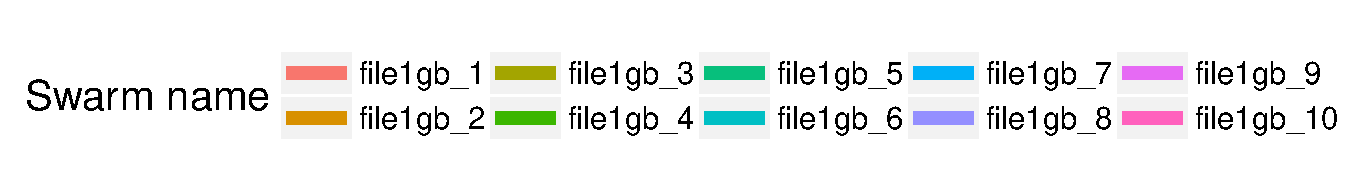
\includegraphics[width=0.8\textwidth]{pics/results/legends.eps}
		\end{subfigure}
		\begin{subfigure}[t]{0.6\textwidth}
			\vspace{-0.5cm}
			\centering
			\includegraphics[width=\textwidth]{pics/results/simple1_sr_notrig.pdf}
			\caption{Seeder ratio policy gain.}
			\label{fig:simplesrnotrig}
		\end{subfigure}
		~
		\begin{subfigure}[t]{0.6\textwidth}
			\vspace{-0.5cm}
			\centering
			\includegraphics[width=\textwidth]{pics/results/simple1_scsr_notrig.pdf}
			\caption{Scoring policy gain.}
			\label{fig:simplescsrnotrig}
		\end{subfigure}
		\caption{The net upload gain of both policies.}
	\end{adjustwidth}
\end{figure} 

In Figure \ref{fig:simplescsrnotrig}, the scoring policy is applied. Unsurprisingly, the trend is similar. This time, the gain is 538 MB, almost twice that of the seeder policy with the same swarm.  Although \texttt{file1gb\_2} returned the highest gain, its upload ratio is not the highest at only 2.99.  The highest ratio is returned by \texttt{file1gb\_7} at 4.91, and the average from all the swarms is 3.718. Average upload speed for this swarm is 94.4 kB/s with 90\% of the observation taking more than 80\% of the maximum upload rate. By these results, it is clear that the factor that limits the credit mining system obtaining higher gain is the maximum upload rate. 

After we observed those, we arrived at three conclusions. First, our hypothesis about the similar choice in this particular experiment on both of the policies is proved to be correct. Although the gain is significantly different, it was not directly caused by the mining system. Instead, it is part of the \bt~protocol, one that builds up the download and upload speed. Second, although the resource may be used to its full capacity as shown in Figure \ref{fig:simplescsrnotrig}, it is entirely possible that it is not used efficiently. This is shown by the inactivity from the other swarms. Net upload gain for other swarms is barely increased in both cases. This locked-up condition is caused by the \textit{libtorrent}'s \textit{share mode} algorithm and its cause and possible solutions already discussed in Section \ref{section:sharemode}. Third, the swarm that gets the highest net upload gain does not necessarily have the highest ratio. As stated in Section \ref{section:filterinetexp}, this is caused by the prospecting mechanism that downloads only a few of the rarest pieces and then uploads those pieces to most of the peers. After downloading these rarest pieces, some of the swarms are not chosen by policy. Therefore, the ratio remains high because there is no downloading activity. 

\subsubsection{The effect of stimulating swarms}
With swarm stimulation, \textit{stale} swarms tend to gain more credits when mined. Figure \ref{fig:simplesrtrig} shows the case for seeder ratio policy and Figure \ref{fig:simplescsrtrig} for scoring policy. We specifically focus on swarm \texttt{file1gb\_1} and \texttt{file1gb\_3} because not only they are the most affected swarms by the stimulation mechanism, but also they have the worst performance among the three in previous experiment. 

\begin{figure}[h]
	\begin{adjustwidth}{-1.5cm}{}
		\begin{subfigure}[t]{1.2\textwidth}
			\centering
			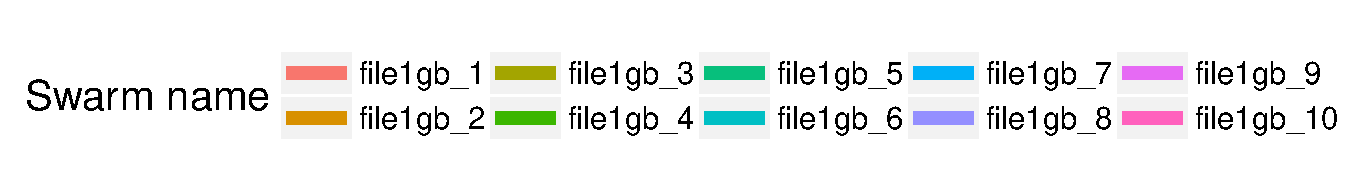
\includegraphics[width=0.8\textwidth]{pics/results/legends.eps}
		\end{subfigure}
		\begin{subfigure}[b]{0.6\textwidth}
			\vspace{-0.2cm}
			\centering
			\includegraphics[width=\textwidth]{pics/results/simple3_sr_trig.pdf}
			\caption{Seeder ratio policy gain with stimulation enabled.}
			\label{fig:simplesrtrig}
		\end{subfigure}
		~
		\begin{subfigure}[b]{0.6\textwidth}
			\vspace{-0.2cm}
			\centering
			\includegraphics[width=\textwidth]{pics/results/simple1_scsr_trig.pdf}
			\caption{Scoring policy gain with stimulation enabled.}
			\label{fig:simplescsrtrig}
		\end{subfigure}
		\caption{The net upload gain of both policies with stimulation enabled.}
	\end{adjustwidth}
\end{figure}

\begin{table}[h]
	\centering
	\caption{Stimulation effect on gained credit.}
	\label{tbl:stimul}
	\begin{adjustwidth}{-1cm}{}
	\begin{tabular}{|c|c|l|l|l|l|}
		\hline
		\multirow{2}{*}{\textbf{Swarm name}} & \multirow{2}{*}{\textbf{Policy}} & \multicolumn{2}{c|}{\textbf{Upload ratio}} & \multicolumn{2}{c|}{\textbf{Net upload gain (in MB)}} \\ \cline{3-6} 
		&  & \textbf{St. Enabled} & \textbf{St. Disabled} & \textbf{St. Enabled} & \textbf{St. Disabled} \\ \hline
		\texttt{file1gb\_1} & Seeder ratio & 3.37 & 1.95 & 148 & 28 \\ \hline
		\texttt{file1gb\_3} & Seeder ratio & 2.88 & 1.95 & 105 & 26 \\ \hline
		\texttt{file1gb\_1} & Scoring & 3.07 & 2.84 & 198 & 77 \\ \hline
		\texttt{file1gb\_3} & Scoring & 3.00 & 3.21 & 134 & 25 \\ \hline
	\end{tabular}
\end{adjustwidth}
\end{table}

Compared to previous results, stale swarms have  their performance increased as shown in Table \ref{tbl:stimul}. From the figure, many bumps that lead to the increasing amount of gain are spotted. In seeder ratio policy, the total stimulant of each swarm is 20 and 12 for \texttt{file1gb\_1} and \texttt{file1gb\_3}, respectively. Also, both upload ratio and net upload gain are significantly increased. This result is in line with our expectations. On the contrary, in scoring policy, the effect of stimulation is not significant. Although upload gain is increased, the ratio is similar to that of when stimulation was disabled. This happened because in the previous scoring policy experiment, most of the resource was already in use. Therefore, we conclude that swarm stimulation works best when the resource in a miner is not fully used, and there are idle swarms in the community.

% 100 swarm for 12, 24. 500 swarm for 24h
\vspace{-0.3cm} 
\section{Comparing obtained gain with prior work}
In this experiment, we will evaluate the result of the proposed system compared to prior work. The comparison experiment run separately for 24 hours on 9 and 10 December 2016 for the prior work and current work, respectively. \textit{Etree.org} will be used as the mining source because the prior version could neither handle other sources nor use the experiment framework in a closed environment. The recommended parameter on the prior work is \textit{SeederRatio} as policy, target ratio is 3, and a 5 minute swarm interval. The result will be shown in Figure \ref{fig:oldetree24}.

For the proposed system, we applied the scoring policy with stimulation enabled. The other configurations will be kept identical with that of the prior work. The result will then be compared to the prior work. We expect that more credit will be gained in this system compared to the prior's one. Figure \ref{fig:newetree24} shows the result of the proposed system. Both experiments run without download/upload rate limit.

%Note that the axis that represents net upload gain in both results is logarithmic.

\begin{figure}[h]
	\begin{adjustwidth}{-1.5cm}{}
		\begin{subfigure}[t]{0.6\textwidth}
			\centering
			\includegraphics[width=\textwidth]{pics/results/b136.pdf}
			\caption{24-hour mining result for current system.}
			\label{fig:newetree24}
		\end{subfigure}
		~
		\begin{subfigure}[t]{0.6\textwidth}
			\centering
			\includegraphics[width=\textwidth]{pics/results/m138.pdf}
			\caption{24-hour mining result for prior's system.}
			\label{fig:oldetree24}
		\end{subfigure}
		\caption{The 24-hour mining result comparison of two systems.}
	\end{adjustwidth}
\end{figure}

The total net upload gain from the prior work is reached 8971 MB. In the other hand, our system can reach 45470 MB as total net upload gain. This shows that with all the features enabled, our system can gain more credits than prior work's. However, we find one similarity. Both of the systems are dominated by only a few swarms. It means that not all of the recent swarms are popular. A popular swarm usually has more leechers, which impacts the overall credit gain. For the main difference, we found two aspects that show that the new credit mining system is better: policy stability and reducing idleness. In the new system, thanks to the investment algorithm, the miners do not need to unnecessarily switch swarms. It shows that the lines tend to be more continuous compared to ones in prior work. When the line is invisible, it means that the particular swarm was not selected in this round. Secondly, it is the idleness of a swarm which is represented in straight horizontal line in the figures. The idle swarm is successfully reduced by enabling stimulation. In the experiment of the proposed system, when net upload gained is more than 500 MB, none of the swarms are idle. On the contrary, some swarms in prior work are idle, even when their upload gain is already high. It can be seen in three straight horizontal lines above the 1000 MB gain.

\vspace{-0.3cm} 
\section{Sustaining user experience on downloading}
\label{section:expprio}
As mentioned in \ref{section:uactivityimpl}, the credit mining system that is implemented within Tribler needs to accommodate user download activity when mining. This experiment will validate that feature. The expectation is that when both credit mining and user download is active, the bandwidth used in user download will remain stable. If only credit mining is active, then the system will maximize the bandwidth if possible. 

The experiment runs in the environment as follows. We launched 40 peers and 4 swarms in a single community. One of the swarms contains a file with size 1 GB and the rest of the swarms have a 2 GB file. Each swarm has 4 dedicated seeders. We then arbitrarily decide the number of downloaders for each swarm. All of the peers have credit mining disabled except the one in which we have our interest. 

At the start, the observed peer activates the credit mining system. In minute 25 of the experiment, this peer intentionally downloads one of the swarm that has 2 GB file size. We call this swarm as the \textit{target} swarm. Then, at minute 120, new peers join the targeted swarm. We will then observe the behavior of our implementation from the peer's perspective. As for comparison, we launch a similar experiment but the observed peer does not activate credit mining system. 

\vspace{-0.4cm}
\begin{figure}[h!]
	
	\begin{subfigure}{\textwidth}
		\includegraphics[width=\textwidth]{pics/results/legends-prio.pdf}
	\end{subfigure}
	\begin{subfigure}{0.6\textwidth}
		\vspace{-0.65cm}
		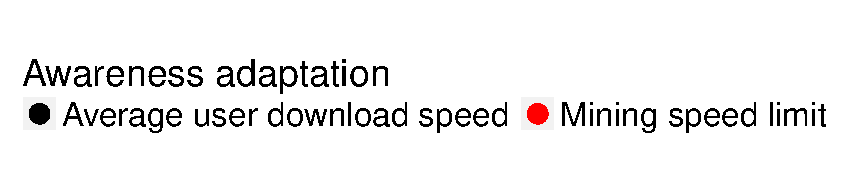
\includegraphics[width=\textwidth]{pics/results/legends-prio2.eps}
	\end{subfigure}
%	\begin{adjustwidth}{-1.5cm}{}
	
	\begin{subfigure}{0.9\textwidth}
		\vspace{-0.2cm}
		\centering
		\includegraphics[width=\textwidth]{pics/results/pr_g2-act2_cpl2.pdf}
	\end{subfigure}
%	\end{adjustwidth}
	\vspace{-0.2cm}
	\caption{The download speed of user download activity and mining activity.}
	\label{fig:cmprio}
\end{figure}

The result in Figure \ref{fig:cmprio} shows the download speed on observed peers. The blue and green line shows user download activity with and without activating credit mining, respectively. Before the new batch of peers arrive, both findings resulted in similar speed constantly in the 150-170 kB/s range. After the new batch of peers arrived (as shown by black vertical line), the speed reaches up to 150 kB/s for both cases. The results match with our expectation that credit mining system has a negligible effect on the overall user experience. 

In the same Figure, the red line is shown as the accumulative download speed for all of the mined swarms except the targeted swarm. Before the user promptly downloads a particular swarm, the mining speed reaches 129 kB/s. After that, it is adjusted to 20-45 kB/s. Totaling both mining and downloading activity download speed resulting more than 200 kB/s, which is 80\% of the total download bandwidth. 

Sometimes, the mining speed is 0 because the credit mining system is in the observation period. In this period, as shown as gray-colored area, the average user activity download speed, as shown with black dots, is examined. Moreover, the mining download limit is marked by red dots. From the results, the trend of user download and mining speed is contradictory. When the user download speed is increased, the credit mining system adjusts its mining speed by allocating lower bandwidth, as shown in the first to second pair of dots. This is also valid in the opposite manner, which is when the download speed is decreased. These results show that the credit mining system is able to run and to adapt with unused bandwidth. 
\vspace{-0.3cm} 
\section{Swarm performance with credit mining}
\label{section:swperf}
After we confidently get a high return gain from the previous results, it is worth finding out what are the effects of credit mining implementation on the community. We expect that credit mining system will increase the swarm's performance. The experiments run with the similar setup and setting as in the Section \ref{section:evalscoring}, except that now we add more than one miner. We also use the scoring policy as default, and enable the swarm stimulation mechanism. The other parameters are left default. 

Figure \ref{fig:swarmnocmperf} shows the average download speed from all of the peers in each of the swarm. In this experiment, no credit mining systems are active. The peers of some of the high-seeded swarms, such as \texttt{file1gb\_8}, \texttt{file1gb\_9}, and \texttt{file1}- -\texttt{gb\_10}, have already reached their maximum download speed. For comparison purpose, we will take this result as a base result in the next experiments.

\begin{figure}[h]
	\centering
	\includegraphics[width=\textwidth]{pics/results/swperf_n2.png}
	\caption{The swarm performance without any credit mining system.}
	\label{fig:swarmnocmperf}
%1   94.57627  exp_3h_swperf_simple_file1gb_1
%4  129.47460  exp_3h_swperf_simple_file1gb_2
%5  147.20364  exp_3h_swperf_simple_file1gb_3
%9  165.74839  exp_3h_swperf_simple_file1gb_4
%3  182.56930  exp_3h_swperf_simple_file1gb_5
%6  199.86998  exp_3h_swperf_simple_file1gb_6
%8  220.01941  exp_3h_swperf_simple_file1gb_7
%10 231.39755  exp_3h_swperf_simple_file1gb_8
%7  232.65703  exp_3h_swperf_simple_file1gb_9
%2  233.83902 exp_3h_swperf_simple_file1gb_10
\end{figure}

%1   exp_3h_swperf_simple_file1gb_1  93.76134  94.57627 -0.8616701
%3   exp_3h_swperf_simple_file1gb_2 168.16871 129.47460 29.8854806
%4   exp_3h_swperf_simple_file1gb_3 185.46871 147.20364 25.9946522
%5   exp_3h_swperf_simple_file1gb_4 196.11774 165.74839 18.3225624
%6   exp_3h_swperf_simple_file1gb_5 218.05894 182.56930 19.4389914
%7   exp_3h_swperf_simple_file1gb_6 210.70760 199.86998  5.4223374
%8   exp_3h_swperf_simple_file1gb_7 221.76209 220.01941  0.7920564
%9   exp_3h_swperf_simple_file1gb_8 232.99379 231.39755  0.6898231
%10  exp_3h_swperf_simple_file1gb_9 231.35478 232.65703 -0.5597267
%2  exp_3h_swperf_simple_file1gb_10 231.79176 233.83902 -0.8754966

Next, we will introduce the credit mining system in the swarms. We start by spawning credit mining system for half of the number of downloaders, which is 25 nodes. Those are dedicated miners that started simultaneously. Figure \ref{fig:swarmcm25perf} shows the average download speed from all the downloaders for each of the swarms. We define the swarm as \textit{covered} by the credit mining if the performance is significantly either increased or dropped, i.e. by more than 5\%. In this experiment, the credit mining covers swarms from \texttt{1gb\_2} to \texttt{1gb\_5}. Compared to the experiment without credit mining, the download speed is increased by at least 18.3\% (\texttt{1gb\_4}) to 29.8\% (swarm \texttt{1gb\_2}). For an unaffected swarm, the speed can decrease up to 0.8\%.

\begin{figure}[h!]
	\centering
	\includegraphics[width=\textwidth]{pics/results/swperf_sc2_25.png}
	\caption{The swarm performance with 25 credit miners in the swarm.}
	\label{fig:swarmcm25perf}
	% mean	
	%	1   93.76134  exp_3h_swperf_simple_file1gb_1
	%	4  168.16871  exp_3h_swperf_simple_file1gb_2
	%	5  185.46871  exp_3h_swperf_simple_file1gb_3
	%	9  196.11774  exp_3h_swperf_simple_file1gb_4
	%	3  218.05894  exp_3h_swperf_simple_file1gb_5
	%	6  210.70760  exp_3h_swperf_simple_file1gb_6
	%	8  221.76209  exp_3h_swperf_simple_file1gb_7
	%	10 232.99379  exp_3h_swperf_simple_file1gb_8
	%	7  231.35478  exp_3h_swperf_simple_file1gb_9
	%	2  231.79176 exp_3h_swperf_simple_file1gb_10
\end{figure}

There are two notable drawbacks when introducing the credit mining system to the swarm, one of which is that the download speed has become unstable. This occurs because of two reasons. First, because of swarm stimulation, there is a higher chance for the miners to become more active on downloading pieces. Second, when switching to a new swarm, miners have incomplete peers information. Therefore, they need to download new pieces to be able to mine. Both reasons are intended to maximize the upload gain. When the miner downloads any piece, it takes the seeder's bandwidth. Therefore, the download speed for other downloaders is decreasing. These factors combined explains the occurrence of instability.

The second drawback is the fact that not all the swarms are boosted by the system. The swarms with a high number of seeders such as swarm \texttt{1gb\_6} and \texttt{1gb\_7} are not boosted. With the way miners prioritize the swarms, only the lowest-seeded swarm will be filled with miners. In other words, there are not enough miners to boost all of the swarms in this experiment.

% Note that the lowest number of seeders gives a worse performance than the base experiment. The reason is that the miner takes the seeder's bandwidth that is supposed to be the downloader's. Because of that, the downloaders get lower speeds. However, miners cannot give back its downloaded pieces to all downloaders in time. In other words, the bottleneck is on the seeder's bandwidth because the seeder cannot deliver the piece fast enough for the miners to distribute the pieces efficiently.
\vspace{-0.3cm} 
\subsection{Varying the number of credit miners}
In this experiment, we will change the number of credit miners in a community. First, we double the number to 50 nodes. The average downloaders' download speed can be seen in Figure \ref{fig:swarmcmperf}. Although the download instability is still present, not only the speed is faster than the 25-miners experiment, it also overcomes the second drawback. Compared to the previous experiment, this shows that the number of miners relates to the boosting coverage of swarms. With 50 miners, it is enough to cover all the possible swarms in this community. Moreover, it also increases the swarm's performance up to 34.6\% (swarm \texttt{1gb\_3}). The lowest and average increasing performance is 3.9\% (swarm \texttt{1gb\_7}) and 17.98\%, respectively.

%The exceptional case of the swarm with a single seeder still holds. 

\begin{figure}[h]
	\begin{subfigure}[h]{\textwidth}
		\centering
		\includegraphics[width=\textwidth]{pics/results/swperf_sc2.png}
		\caption{The swarm performance with 50 credit miners in the swarm.}
		\label{fig:swarmcmperf}
		%		1   90.44611  exp_3h_swperf_simple_file1gb_1 -4.36701510854678
		%		4  174.32050  exp_3h_swperf_simple_file1gb_2 34.6368322435443
		%		5  197.69961  exp_3h_swperf_simple_file1gb_3 34.3034791802702
		%		9  216.80348  exp_3h_swperf_simple_file1gb_4 30.8027667719729
		%		3  213.11578  exp_3h_swperf_simple_file1gb_5 16.7314438955509
		%		6  219.55919  exp_3h_swperf_simple_file1gb_6 9.8510091410426
		%		8  228.68752  exp_3h_swperf_simple_file1gb_7 3.93970241080095
		%		10 230.21745  exp_3h_swperf_simple_file1gb_8 -0.509988113530142
		%		7  228.38337  exp_3h_swperf_simple_file1gb_9 -1.83689269995409
		%		2  228.60623 exp_3h_swperf_simple_file1gb_10 -2.23777451684496
		
	\end{subfigure}
	\begin{subfigure}[h]{\textwidth}
		\centering
		\includegraphics[width=\textwidth]{pics/results/swperf_sc1_10.png}
		\caption{The swarm performance with 10 credit miners in the swarm.}
		\label{fig:swarmcm10perf}
	\end{subfigure}
	%	          average_speed   filename 
	%	          1   93.84661  file1gb_1	
	%	          4  156.09825  file1gb_2
	%	          5  165.20124  file1gb_3
	%	          9  179.36101  file1gb_4
	%	          3  185.69509  file1gb_5
	%	          6  204.56280  file1gb_6
	%	          8  221.31673  file1gb_7
	%	          10 228.48779  file1gb_8
	%	          7  233.63073  file1gb_9
	%	          2  232.48323  file1gb_10
	\caption{The swarm performance of different number of credit miners in the swarm.}
\end{figure}

Second, we also conducted an experiment with fewer miners. In this case, the number of credit miners is set to 10 nodes. From Figure \ref{fig:swarmcm10perf}, it is shown that the coverage is lessened. Now, more swarms (from \texttt{1gb\_5} to \texttt{1gb\_10}) are not boosted by the miners. The average speed is slightly higher than that of the base experiment, but lower than the 25-miners experiment. The highest performance increase is on the swarm \texttt{1gb\_2} with 20.5\%, and the lowest is on the swarm \texttt{1gb\_4} with 8.21\%. This emphasizes the positive relation between the number of miners, boosting coverage, and swarms' performance.


\subsection{The effect of swarm stimulation}
\begin{figure}[h!]
	\centering
	\includegraphics[width=\textwidth]{pics/results/swperf_sc1_notrig.png}
	\caption{The swarm performance with 25 credit miners (without stimulation) in the swarm.}
	\label{fig:swarmcm25perfnotrig}
	%		avg_dl_speed fname
	%	1   93.68527  file1gb_1
	%	4  138.86226  file1gb_2
	%	5  164.62305  file1gb_3
	%	9  212.60381  file1gb_4
	%	3  215.89967  file1gb_5
	%	6  203.22903  file1gb_6
	%	8  216.89871  file1gb_7
	%	10 228.13082  file1gb_8
	%	7  233.89741  file1gb_9
	%	2  232.99496 file1gb_10
\end{figure}

Our next experiment is conducted to understand the effect of swarm stimulation on the community. As shown before (in Section \ref{section:resultgain}), swarm stimulation can increase the credit gain for the user. A notable difference from this experiment is that the average speed instability is gone, as can be seen in Figure \ref{fig:swarmcm25perfnotrig}. However, as a trade-off, the average speed is slightly lower on the boosted swarm. Compared to the 25-miners experiment, only swarm \texttt{1gb\_4} is better with 8\% increased download speed. The rest have their performance decreased starting from 1\% (\texttt{file1gb\_5}) to 17\% (\texttt{file1gb\_2}). Even so, it is still better than the base experiment. Swarm \texttt{file1gb\_4} improves as much as 28\%, and swarm \texttt{file1gb\_2} still improves by 7.25\%. Another disadvantage is that on the lower-seeded swarms, namely \texttt{1gb\_1} and \texttt{1gb\_2}, they have negligible difference compared to the base experiment's, especially in the latter half of the experiment. Therefore, the coverage of the boosted swarm is also reduced because of the existence of stale swarms. 

Swarm stimulation is the major cause of the instability of the peers' download speed. When it is active, it will consume the bandwidth from
all the peers. Thus, the swarm performance is decreasing. After it finishes downloading the pieces, it will increase the swarm performance by immediately returning the bandwidth it consumed back to the swarms in an equal or higher amount. We also find that stimulating swarm on a very few seeders is counterproductive. Compared to 25-miners experiment, only the performance for \texttt{1gb\_4} and  \texttt{1gb\_5} are equal or increased. From the community's perspective, swarm stimulation mechanism seems to negate the benefits of credit mining system for some swarms.

%However, we argue that stimulate swarm with very few seeders is counterproductive. Although the stimulation can be widely enabled on all the swarms which gives very little drawback, it seems to be unsuitable for some swarms. 

% CONCLUSIONS AND FUTURE WORK
\chapter{Conclusions and Future Work}
\label{chp:conclusionsandfuturework}

\section{Conclusions}
This thesis aims to solve \bt~supply and demand misalignment introduced by the freeriders. We devised an automatic mechanism to effectively gain credit in the existing credit system. We showed that it benefits both individual and communities. The user can gain the credit without a need to seed for a long time. The swarms in the community also can get higher download speed and content availability.

We then proposed \textit{credit mining system}, an autonomous system to download pieces from selected swarms in order to gain high upload ratio in the future. It can run on top of the traditional credit system that already widely implemented in both private and public communities. Credit mining system finds swarms with high return potential, picks the rarest pieces, and uploads those to the community using all the available bandwidth.

We focus on the investment algorithm which is the core of credit mining. Two stage of the algorithm were presented. Both stages are important. \textit{Prospecting} stage filters a huge number of swarm while keeping resilience by not solely depending on a centralized tracker. \textit{Mining} stage only selects best swarms that have high gain potential. If necessary, it also stops problematic or low potential swarms. We also proposed \textit{scoring} policy, a highly customizable method to quantify swarms into a score that can be compared to each other and reduces possible identical result.

Credit mining system now is fully integrated with Tribler. When enabled, it is tailored to not interfere with users activity on downloading. Provided with accessible GUI, a user can easily interact with the system to start investing. Before the system is implemented, it has passed several tests and proved to be stable on cross-platform. All the components designed to not hinder user experience while credit mining system is active.

The performance of credit mining system is fulfilled our expectation. All the components were doing their tasks properly. Prospecting is both fast and accurate to find and filter swarms on the Internet. Scoring policy successfully selects the most undersupplied swarms and surpasses previous policy accuracy. Moreover, it also stops both saturated and low potential swarm. With stimulating enabled, most of the time, the system use a large portion (80\%) of its resources. The upload/download ratio can reach up to 4.91 with average 3.71 although the target was only 2.0. After making the comparison, the current system can gain more credit than in prior work. We also showed that credit miners have a good impact on the community as a whole. With the number of miners is half of the peers, it can boost more than half of swarms in a particular community by up to 29\%. Increasing the number of miners can increase the swarm coverage as well as the average peers' download speed.

\section{Future Work}
Currently, credit miners still see other miners as a normal peer. There might be a case where a miner seeds to another miner, which is unnecessary. The key problem of "Co-Investors" is to recognize and utilize the existence of other miners. With recognizing other miners, investment can be more selective. There is less need to boost a swarm if there are already miners in there, for example. 

Although we proposed the scoring policy in this thesis, the optimal \textit{multipliers} to reach the highest gain possible is still unknown. With many parameters, the study to find the weight and importance of those parameters is desired. Furthermore, this policy can be extended by adding more parameters by adopting the same calculation method.

Another aspect that still unknown is whether using different policies for different swarms is beneficial. Currently, the policy can not be changed, and all swarms need to comply with a single policy. Moreover, as we shown in the previous chapter, not all swarms suitable to be stimulated. The \textit{partial mining} mechanism is a method to apply different policies and optimizations to different swarm in order to get highest credit gain possible. 

% BIBLIOGRAPHY
%\bibliographystyle{bib/latex8}
\bibliographystyle{bib/IEEEtranN} % changed latex8, I think its compatible
\bibliography{bib/bibliography}

%\appendix

%\chapter{APPENDIX }
\label{app:as}
Appendix body


%\begin{table}[h]
%	\centering
%	\caption{Probability swarm chooser}
%	\begin{adjustwidth}{-2.5cm}{}
%		\begin{tabular}{|c|p{1.5cm}|p{1.5cm}|p{1.5cm}|p{1.5cm}||c|p{1.5cm}|p{1.5cm}|p{1.5cm}|p{1.5cm}|}
%			\hline
%			\rowcolor[HTML]{EFEFEF} 
%			No. & \textit{sc} top 3 (top 6) & \textit{sr} top 3 (top 6) & \textit{sc} on top session & \textit{sr} on top session & No. & \textit{sc} top 3 (top 6) & \textit{sr} top 3 (top 6) & \textit{sc} on top session & \textit{sr} on top session \\ \hline
%			1 & 0  (0) & 0  (0) & 0 & 0 & 19 & 1  (1) & 1  (1) & 1 & 2\\ \hline
%			2 & 0  (0) & 1  (1) & 0 & 1 & 20 & 1  (1) & 1  (1) & 2 & 2\\ \hline
%			3 & 0  (0) & 1  (1) & 0 & 1 & 21 & 1  (2) & 1  (1) & 2 & 2\\ \hline
%			4 & 1  (2) & 1  (1) & 2 & 2 & 22 & 1  (2) & 1  (1) & 2 & 2\\ \hline
%			5 & 1  (2) & 1  (1) & 2 & 1 & 23 & 1  (2) & 1  (1) & 2 & 2\\ \hline
%			6 & 2  (3) & 1  (1) & 3 & 1 & 24 & 1  (1) & 1  (0) & 2 & 2\\ \hline
%			7 & 2  (3) & 1  (1) & 3 & 1 & 25 & 1  (0) & 1  (0) & 2 & 2\\ \hline
%			8 & 1  (2) & 1  (1) & 2 & 2 & 26 & 1  (0) & 1  (0) & 1 & 2\\ \hline
%			9 & 2  (3) & 1  (1) & 3 & 1 & 27 & 1  (0) & 1  (0) & 1 & 1\\ \hline
%			10 & 2  (3) & 1  (1) & 3 & 1 & 28 & 1  (0) & 1  (0) & 1 & 1\\ \hline
%			11 & 2  (3) & 1  (1) & 3 & 1 & 29 & 1  (0) & 1  (0) & 1 & 1\\ \hline
%			12 & 2  (3) & 1  (1) & 3 & 1 & 30 & 1  (0) & 1  (0) & 1 & 1\\ \hline
%			13 & 2  (3) & 1  (1) & 3 & 1 & 31 & 1  (0) & 1  (0) & 1 & 1\\ \hline
%			14 & 1  (2) & 1  (1) & 2 & 1 & 32 & 1  (0) & 1  (0) & 1 & 1\\ \hline
%			15 & 1  (1) & 1  (1) & 2 & 2 & 33 & 0  (0) & 1  (0) & 0 & 1\\ \hline
%			16 & 2  (2) & 1  (1) & 2 & 1 & 34 & 0  (0) & 1  (0) & 0 & 1\\ \hline
%			17 & 1  (2) & 1  (1) & 2 & 1 & 35 & 0  (0) & 1  (0) & 0 & 1\\ \hline
%			18 & 2  (1) & 1  (0) & 2 & 2 & 36 & 0  (0) & 0  (0) & 0 & 0\\ \hline
%		\end{tabular}
%	\end{adjustwidth}
%\end{table}

%Alternative : 

%\begin{table}[h]
%	\centering
%	\caption{Probability swarm chooser (percentage)}
%	\begin{adjustwidth}{-3cm}{}
%		\begin{tabular}{|c|p{1.8cm}|p{1.8cm}|p{1.3cm}|p{1.3cm}||c|p{1.8cm}|p{1.8cm}|p{1.3cm}|p{1.3cm}|}
%			\hline
%			\rowcolor[HTML]{EFEFEF} 
%			Round & \textit{sc} top 3 (top 6) & \textit{sr} top 3 (top 6) & \textit{sc} on top session & \textit{sr} on top session & Round & \textit{sc} top 3 (top 6) & \textit{sr} top 3 (top 6) & \textit{sc} on top session & \textit{sr} on top session \\ \hline
%			1 & 0\%(0\%) & 0\%(0\%) & 0\% & 0\% & 19 & 33\%(33\%) & 33\%(33\%) & 33\% & 67\%\\\hline
%			2 & 0\%(0\%) & 33\%(33\%) & 0\% & 33\% & 20 & 33\%(33\%) & 33\%(33\%) & 67\% & 67\%\\\hline
%			3 & 0\%(0\%) & 33\%(33\%) & 0\% & 33\% & 21 & 33\%(67\%) & 33\%(33\%) & 67\% & 67\%\\\hline
%			4 & 33\%(67\%) & 33\%(33\%) & 67\% & 67\% & 22 & 33\%(67\%) & 33\%(33\%) & 67\% & 67\%\\\hline
%			5 & 33\%(67\%) & 33\%(33\%) & 67\% & 33\% & 23 & 33\%(67\%) & 33\%(33\%) & 67\% & 67\%\\\hline
%			6 & 67\%(100\%) & 33\%(33\%) & 100\% & 33\% & 24 & 33\%(33\%) & 33\%(0\%) & 67\% & 67\%\\\hline
%			7 & 67\%(100\%) & 33\%(33\%) & 100\% & 33\% & 25 & 33\%(0\%) & 33\%(0\%) & 67\% & 67\%\\\hline
%			8 & 33\%(67\%) & 33\%(33\%) & 67\% & 67\% & 26 & 33\%(0\%) & 33\%(0\%) & 33\% & 67\%\\\hline
%			9 & 67\%(100\%) & 33\%(33\%) & 100\% & 33\% & 27 & 33\%(0\%) & 33\%(0\%) & 33\% & 33\%\\\hline
%			10 & 67\%(100\%) & 33\%(33\%) & 100\% & 33\% & 28 & 33\%(0\%) & 33\%(0\%) & 33\% & 33\%\\\hline
%			11 & 67\%(100\%) & 33\%(33\%) & 100\% & 33\% & 29 & 33\%(0\%) & 33\%(0\%) & 33\% & 33\%\\\hline
%			12 & 67\%(100\%) & 33\%(33\%) & 100\% & 33\% & 30 & 33\%(0\%) & 33\%(0\%) & 33\% & 33\%\\\hline
%			13 & 67\%(100\%) & 33\%(33\%) & 100\% & 33\% & 31 & 33\%(0\%) & 33\%(0\%) & 33\% & 33\%\\\hline
%			14 & 33\%(67\%) & 33\%(33\%) & 67\% & 33\% & 32 & 33\%(0\%) & 33\%(0\%) & 33\% & 33\%\\\hline
%			15 & 33\%(33\%) & 33\%(33\%) & 67\% & 67\% & 33 & 0\%(0\%) & 33\%(0\%) & 0\% & 33\%\\\hline
%			16 & 67\%(67\%) & 33\%(33\%) & 67\% & 33\% & 34 & 0\%(0\%) & 33\%(0\%) & 0\% & 33\%\\\hline
%			17 & 33\%(67\%) & 33\%(33\%) & 67\% & 33\% & 35 & 0\%(0\%) & 33\%(0\%) & 0\% & 33\%\\\hline
%			18 & 67\%(33\%) & 33\%(0\%) & 67\% & 67\% & 36 & 0\%(0\%) & 0\%(0\%) & 0\% & 0\%\\\hline
%		\end{tabular}
%	\end{adjustwidth}
%\end{table}

scoring policy in general similar with sederpolicy. But with considering other factors as well.

in selecting the policy only, the behaviour will similar. Except in edge conditions -> with different availability. Similar seeder ratio.
=========================================
choosing best swarm
case 1
1. different : seederratio -> expect : similar performance (upload gain) for sr and sc
scatter, gain graph
sc gain ~= sr gain

case 2
2. different : availability -> sc should gather more. seederratio sama, ukuran file beda -> different availability
scatter, gain graph
sc gain > sr gain

mention kalau complex experiment ada di akhir (lebih lama)
DISABLE TRIGGER AND BLACKLIST
=======================================

increasing Net upload gain

scoring policy
with trigger < 1.5 times
blacklist 40mins - 1h recov


Statistics (scoring vs seeder ratio): 
\begin{enumerate}
	\item Strictly larger Top 3  : 9 (25 \% better)
	\item Strictly larger Top 6  : 18 (50 \% better)
	\item Strictly larger top session  : 11
	\item larger or equal Top 3  : 32 (cover 88 \%)
	\item larger or equal Top 6  : 35 (cover 97 \%)
	\item larger or equal top session  : 30
\end{enumerate}

%\begin{itemize}
%	\item old one use \textit{net upload gain}. etree.org for two day (48 hour). Test with 1 and half day.
%	\item Best old one is SeederRatio with 5 minute with 1 ratio (gain higher upload gain). Optimal : 3 ratio.
%	\item CM+boost : seederratio, 5 minutes, 3 ratio
%	\item mihai 136 12 hour. runs first. 6dec
%	\item cm 133. 12 hour. runs second. 8dec
%	\item mihai 137, cm 134 : 12 hour. In parallel
%	\item mihai 138 -> cm 136 24h
%	\item mihai 139 & 137 24h par
%\end{itemize}

\begin{verbbox}
@0:0 set_master_member 307e....5177
@0:2 start_dispersy {1-155}
@0:20 start_session
@0:60 online
@0:60 reset_dispersy_statistics
@0:60 annotate start-experiment
# 1 : creator (seeder)
# 2-12 : dedicated seeder
# 13-81 : peers
# 81 - 85 : flashcrowd all scenario
@0:60 create {1}
@0:61 join {2-20}
@0:62 publish file1gb_1 1524288001 {1}
@0:63 join {21-40}
@0:64 join {41-55}
@0:65 publish file1gb_2 1524288002 {2}
@0:66 publish file1gb_3 1524288003 {3}
@0:67 publish file1gb_4 1524288004 {4}
@0:68 publish file1gb_5 1524288005 {5}
@0:69 publish file1gb_6 1524288006 {6}
@0:70 publish file1gb_7 1524288007 {7}
@0:71 publish file1gb_8 1524288008 {8}
@0:72 publish file1gb_9 1524288009 {9}
@0:73 publish file1gb_10 1524288010 {10}
@5:105 setup_seeder file1gb_2 1524288002 {11}
@5:106 setup_seeder file1gb_3 1524288003 {12-13}
@5:107 setup_seeder file1gb_4 1524288004 {14-16}
@5:108 setup_seeder file1gb_5 1524288005 {17-20}
@5:109 setup_seeder file1gb_6 1524288006 {21-25}
@5:110 setup_seeder file1gb_7 1524288007 {26-31}
@5:111 setup_seeder file1gb_8 1524288008 {32-38}
@5:112 setup_seeder file1gb_9 1524288009 {39-46}
@5:113 setup_seeder file1gb_10 1524288010 {47-55}
@5:114 join {56-105}
@5:115 join {106-155}
# wave 1
@10:12 start_download file1gb_1 {56-60}
@10:12 start_download file1gb_2 {61-65}
@10:12 start_download file1gb_3 {66-70}
@10:12 start_download file1gb_4 {71-75}
@10:12 start_download file1gb_5 {76-80}
@10:12 start_download file1gb_6 {81-85}
@10:12 start_download file1gb_7 {86-90}
@10:12 start_download file1gb_8 {91-95}
@10:12 start_download file1gb_9 {96-100}
@10:12 start_download file1gb_10 {101-105}
# # @20:0 set_boost_settings boosting.ini.1 {106-155}
@20:2 start_boosting {106-155}
@20:3 add_source joinedchannel {106-155}
@2:58:0 reset_dispersy_statistics
@2:59:0 stop
\end{verbbox}



\end{document}

